% !TEX program = lualatex
\documentclass[A4,svgnames,9pt,aspectratio=169]{beamer}

\usepackage[utf8]{inputenc}
\usepackage{amsmath,amssymb,amsfonts}
\usepackage{mathtools}
\usepackage{bm}
\usepackage{graphicx}
\usepackage{caption}
\usepackage{booktabs}
\usepackage{colortbl}
\usepackage{tikz}
\usetikzlibrary{positioning, shapes, arrows.meta, calc}

\hypersetup{
   allcolors=rouge_inria,
   pdfauthor   = {Louis Hauseux},
   pdftitle    = {De l'intérêt des bibliothèques de geometry processing puissantes pour un clustering hiérarchique fin : CGAL, Geogram, etc.},
   pdfsubject  = {Présentation à Bruno Lévy},
   pdfkeywords = {Louis Hauseux, clustering, Delaunay, percolation, optimal transport}
}

\title[Geometry Processing \& Clustering]{\large De l'intérêt des bibliothèques de \emph{geometry processing} puissantes\\[2pt] pour un clustering hiérarchique fin : CGAL, Geogram, \emph{etc.}\\[6pt] \normalsize \normalfont Et ce qui leur manque encore pour passer aux interactions d’ordre supérieur...}
\subtitle{\small Présentation à \href{https://brunolevy.github.io/}{Bruno \textsc{Lévy}} (Univ. Paris-Saclay, Inria éq. \href{https://team.inria.fr/parma/}{\textsc{ParMa}}, CNRS, Lab. Math. Orsay)}
\date[juin 2026]{Juin 2026}
\author[L. Hauseux]{%
   \small Louis \textsc{Hauseux} (Inria Sophia Antipolis, bourse 3IA--DS4H d'Université Côte d'Azur) \\[3pt]
   \footnotesize Encadré par \href{https://www-sop.inria.fr/members/Konstantin.Avratchenkov/me.html}{Konstantin \textsc{Avrachenkov}} (\textsc{Neo}) \& \href{https://www-sop.inria.fr/members/Josiane.Zerubia/index-eng.html}{Josiane \textsc{Zerubia}} (\textsc{Ayana})
}
\institute{Saclay}

\usetheme{inria}
\setbeamertemplate{bibliography item}[text]


\setbeamertemplate{footnote}{%
  \hspace*{0.6cm}%
  \raisebox{8pt}{%
    \usebeamerfont{footnote}\usebeamercolor[fg]{footnote}%
    \insertfootnotemark~\insertfootnotetext%
  }%
}

\colorlet{inria-bleu}{inria-2024-bleu-azur}

\newcounter{tocsectioncounter}
\renewcommand{\contentsname}{Plan}
\setbeamertemplate{section in toc}{%
    \vspace*{2ex}%
    \setcounter{tocsectioncounter}{\inserttocsectionnumber}%
    \textcolor{inria-noir}{\textbf{\Roman{tocsectioncounter})~\inserttocsection}}%
}

\begin{document}

% Page de titre
\frame{\titlepage}

% Plan
\begin{frame}{Plan}
  \tableofcontents
\end{frame}

\section{Clustering : des statistiques aux (hyper)graphes}
\frame{\sectionpage}

\begin{frame}{Clustering sur données euclidiennes $\mathcal{X} \subset \mathbb{R}^d$}
    \begin{center}
        \large
        \textbf{Modèle de \textsc{Hartigan}} \cite{hartigan81} : \textbf{Amas de forte densité} (\emph{high-density clusters})
    \end{center}
    
    \vspace{0.4cm}
    
    \begin{center}
        \begin{tikzpicture}[every node/.style={inner sep=0}]
            % Données brutes
            \node (raw) [draw=gray!30, line width=1.5pt, inner sep=2pt, label={[label distance=8pt]below:{\small Données brutes $\mathcal{X}$}}] 
                {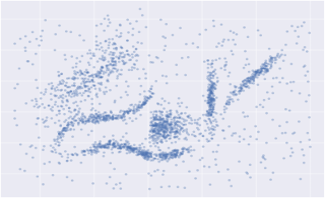
\includegraphics[width=0.22\textwidth]{../Img_presentation_BrunoLevy/Nuage2D.png}};
                
            % Données classées
            \node (clustered) at (6.8, 0) [draw=inria-rouge, line width=1.5pt, inner sep=2pt, label={[label distance=8pt]below:{\small Amas de forte densité}}] 
                {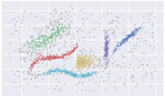
\includegraphics[width=0.22\textwidth]{../Img_presentation_BrunoLevy/Nuage2D_HDBSCAN.png}};
                
            % Flèche grasse au milieu
            \draw[-{Latex[length=10pt, width=10pt]}, line width=5pt, color=gray!40] (2.0, 0) -- (4.8, 0);
            
            % Roues dentées au-dessus de la flèche
            \node (gears) at (3.4, 0.75) {
\includegraphics[width=0.07\textwidth]{imgs/roues_dentee.jpeg}};
            
            % Nom de l'algo en-dessous
            \node (algo) at (3.4, -0.9) [align=center] {\small \textbf{HDBSCAN}\footnotemark[1] \cite{HDBSCAN, HDBSCAN2017}};
        \end{tikzpicture}
    \end{center}
    \footnotetext[1]{Hierarchical Density-Based Spatial Clustering of Applications with Noise}
\end{frame}

\begin{frame}{Quelques exemples}
    \begin{center}
        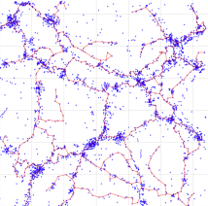
\includegraphics[height=4.5cm]{../Img_presentation_BrunoLevy/FilamentsGalaxie.png}
        
        \vspace{0.5cm}
        \normalsize \textbf{Cosmologie 3D} : filaments cosmiques \cite{BibiMenton}
    \end{center}
\end{frame}

\begin{frame}{Quelques exemples}
    \begin{center}
        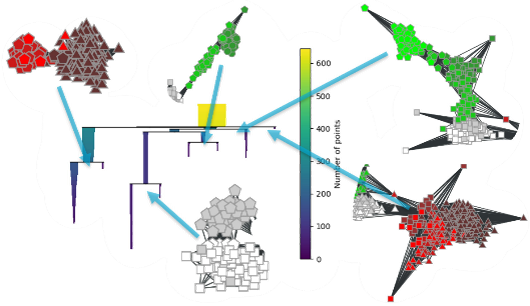
\includegraphics[height=4.0cm]{../Img_presentation_BrunoLevy/CondenseTree_OliveOil_HGP.png}
            
        \vspace{0.5cm}
        \normalsize \textbf{Classification d'huiles d'olive italiennes} \cite{tourr} ($\mathcal{X} \subset \mathbb{R}^8$) : résultat hiérarchique \cite{BibiLyon, BibiAppliedNetworkScience}
    \end{center}
\end{frame}

\begin{frame}{Modèle de \textsc{Hartigan} : hiérarchie des amas de forte densité}
    \begin{columns}[onlytextwidth]
        \begin{column}{0.48\textwidth}
            \begin{center}
                \textbf{Ensemble de niveau} $\{f \ge \lambda\}$
                
                \vspace{0.3cm}
                \begin{tikzpicture}[xscale=0.95, yscale=0.95]
                    \useasboundingbox (-0.8, -0.4) rectangle (6.2, 4.2);
                    \only<1>{\pgfmathsetmacro{\lambdaval}{2.6}}
                    \only<2>{\pgfmathsetmacro{\lambdaval}{1.75}}
                    \only<3>{\pgfmathsetmacro{\lambdaval}{1.1}}
                    \only<4>{\pgfmathsetmacro{\lambdaval}{0.4}}
                    
                    % Axis
                    \draw[->, >=stealth] (0,0) -- (0,4) node[left=5pt, midway, rotate=90] {$f$};
                    
                    % Shaded areas above \lambdaval
                    \begin{scope}
                        \clip (0,\lambdaval) rectangle (6,4);
                        \fill[inria-bleu!20] (0.2,0) -- (0.2, 0.2) .. controls (0.7,0.2) and (0.9,2.0) .. (1.2,2.0)
                            .. controls (1.5,2.0) and (1.6,0.9) .. (1.8,0.9)
                            .. controls (2.0,0.9) and (2.2,1.5) .. (2.4,1.5)
                            .. controls (2.5,1.5) and (2.6,1.3) .. (2.7,1.3)
                            .. controls (2.9,1.3) and (3.1,3.2) .. (3.4,3.2)
                            .. controls (3.7,3.2) and (3.9,0.6) .. (4.2,0.6)
                            .. controls (4.4,0.6) and (4.6,1.3) .. (4.8,1.3)
                            .. controls (5.0,1.3) and (5.4,0.2) .. (5.8,0) -- (5.8,0) -- cycle;
                    \end{scope}
                    
                    % Density curve f(x)
                    \draw[line width=1.5pt, color=inria-bleu] (0.2, 0.2) .. controls (0.7,0.2) and (0.9,2.0) .. (1.2,2.0)
                        .. controls (1.5,2.0) and (1.6,0.9) .. (1.8,0.9)
                        .. controls (2.0,0.9) and (2.2,1.5) .. (2.4,1.5)
                        .. controls (2.5,1.5) and (2.6,1.3) .. (2.7,1.3)
                        .. controls (2.9,1.3) and (3.1,3.2) .. (3.4,3.2)
                        .. controls (3.7,3.2) and (3.9,0.6) .. (4.2,0.6)
                        .. controls (4.4,0.6) and (4.6,1.3) .. (4.8,1.3)
                        .. controls (5.0,1.3) and (5.4,0.2) .. (5.8,0);
                        
                    % Dashed level line \lambdaval
                    \draw[dashed, line width=1pt] (0,\lambdaval) -- (6,\lambdaval);
                    
                    % Peaks and Valleys dots
                    \fill[green!60!black] (1.2,2.0) circle (2.5pt);
                    \fill[green!60!black] (2.4,1.5) circle (2.5pt);
                    \fill[green!60!black] (3.4,3.2) circle (2.5pt);
                    \fill[green!60!black] (4.8,1.3) circle (2.5pt);
                    \fill[inria-rouge] (1.8,0.9) circle (2.5pt);
                    \fill[inria-rouge] (2.7,1.3) circle (2.5pt);
                    \fill[inria-rouge] (4.2,0.6) circle (2.5pt);
                    
                    % Legend
                    \draw[line width=1.5pt, color=inria-bleu] (4.0, 3.7) -- (4.6, 3.7) node[right=3pt] {\small $f$};
                    \draw[dashed, line width=1pt] (4.0, 3.3) -- (4.6, 3.3) node[right=3pt] {\small $\lambda$};
                    
                    % Blue bars at the bottom
                    \only<1>{
                        \draw[inria-bleu, line width=4pt] (3.1, -0.15) -- (3.7, -0.15);
                    }
                    \only<2>{
                        \draw[inria-bleu, line width=4pt] (1.0, -0.15) -- (1.4, -0.15);
                        \draw[inria-bleu, line width=4pt] (2.9, -0.15) -- (4.0, -0.15);
                    }
                    \only<3>{
                        \draw[inria-bleu, line width=4pt] (0.7, -0.15) -- (1.6, -0.15);
                        \draw[inria-bleu, line width=4pt] (1.9, -0.15) -- (4.1, -0.15);
                        \draw[inria-bleu, line width=4pt] (4.5, -0.15) -- (5.1, -0.15);
                    }
                    \only<4>{
                        \draw[inria-bleu, line width=4pt] (0.4, -0.15) -- (5.5, -0.15);
                    }
                \end{tikzpicture}
            \end{center}
        \end{column}
        
        \begin{column}{0.48\textwidth}
            \begin{center}
                \textcolor{inria-rouge}{\textbf{Arbre hiérarchique}}
                
                \vspace{0.3cm}
                \begin{tikzpicture}[xscale=0.95, yscale=0.95]
                    \useasboundingbox (-0.8, -0.4) rectangle (6.2, 4.2);
                    
                    % Tree branches
                    \only<1>{
                        \draw[inria-rouge, line width=1.5pt] (3.4, 3.2) -- (3.4, 2.6);
                        \node[above] at (3.4, 3.2) {\small $C_1$};
                    }
                    \only<2>{
                        \draw[inria-rouge, line width=1.5pt] (3.4, 3.2) -- (3.4, 1.75);
                        \node[above] at (3.4, 3.2) {\small $C_1$};
                        \draw[inria-rouge, line width=1.5pt] (1.2, 2.0) -- (1.2, 1.75);
                        \node[above] at (1.2, 2.0) {\small $C_2$};
                    }
                    \only<3>{
                        \draw[inria-rouge, line width=1.5pt] (1.2, 2.0) -- (1.2, 1.1);
                        \node[above] at (1.2, 2.0) {\small $C_2$};
                        
                        \draw[inria-rouge, line width=1.5pt] (4.8, 1.3) -- (4.8, 1.1);
                        \node[above] at (4.8, 1.3) {\small $C_5$};
                        
                        \draw[inria-rouge, line width=1.5pt, rounded corners=4pt] (2.4, 1.5) -- (2.4, 1.3) -- (2.9, 1.3) -- (2.9, 1.1);
                        \node[above] at (2.4, 1.5) {\small $C_3$};
                        
                        \draw[inria-rouge, line width=1.5pt, rounded corners=4pt] (3.4, 3.2) -- (3.4, 1.3) -- (2.9, 1.3) -- (2.9, 1.1);
                        \node[above] at (3.4, 3.2) {\small $C_1$};
                        
                        \node[above=2pt] at (2.9, 1.3) {\small $C_4$};
                    }
                    \only<4>{
                        % Branch C3 -> Trunk C4 -> Merge 2 -> Trunk C6 -> Merge 3 -> Trunk C7
                        \draw[inria-rouge, line width=1.5pt, rounded corners=4pt] (2.4, 1.5) -- (2.4, 1.3) -- (2.9, 1.3) -- (2.9, 0.9) -- (2.05, 0.9) -- (2.05, 0.6) -- (3.42, 0.6) -- (3.42, 0.4);
                        \node[above] at (2.4, 1.5) {\small $C_3$};
                        \node[above=2pt] at (2.9, 1.3) {\small $C_4$};
                        
                        % Branch C1 -> Merge 1 -> Trunk C4 -> Merge 2 -> Trunk C6 -> Merge 3 -> Trunk C7
                        \draw[inria-rouge, line width=1.5pt, rounded corners=4pt] (3.4, 3.2) -- (3.4, 1.3) -- (2.9, 1.3) -- (2.9, 0.9) -- (2.05, 0.9) -- (2.05, 0.6) -- (3.42, 0.6) -- (3.42, 0.4);
                        \node[above] at (3.4, 3.2) {\small $C_1$};
                        
                        % Branch C2 -> Merge 2 -> Trunk C6 -> Merge 3 -> Trunk C7
                        \draw[inria-rouge, line width=1.5pt, rounded corners=4pt] (1.2, 2.0) -- (1.2, 0.9) -- (2.05, 0.9) -- (2.05, 0.6) -- (3.42, 0.6) -- (3.42, 0.4);
                        \node[above] at (1.2, 2.0) {\small $C_2$};
                        \node[above=2pt] at (2.05, 0.9) {\small $C_6$};
                        
                        % Branch C5 -> Merge 3 -> Trunk C7
                        \draw[inria-rouge, line width=1.5pt, rounded corners=4pt] (4.8, 1.3) -- (4.8, 0.6) -- (3.42, 0.6) -- (3.42, 0.4);
                        \node[above] at (4.8, 1.3) {\small $C_5$};
                        
                        \node[above=2pt] at (3.42, 0.6) {\small $C_7$};
                    }
                \end{tikzpicture}
            \end{center}
        \end{column}
    \end{columns}
\end{frame}

\begin{frame}{Clustering sur données euclidiennes $\mathcal{X} \subset \mathbb{R}^d$ : estimation}
    \vspace{1.0cm}
    \begin{center}
        \begin{tikzpicture}[xscale=1.2, yscale=1.2]
            \useasboundingbox (-1,-3) rectangle (8,2);
            
            \node (unknown) at (0, 0) [align=center] {\huge $f$ inconnue};
            
            % Thick gray arrow
            \draw[-{Latex[length=8pt, width=8pt]}, line width=4.5pt, color=gray!30] (1.8, 0) -- (3.6, 0);
            
            \node (estimation) at (5.8, 0) [align=center] {\huge \textbf{Estimation} $\widehat{f}$};
            
            \node (expensive) at (5.8, -0.85) [align=center] {
                \normalsize Méthodes naïves coûteuses\\
                \small (discrétisation de $\mathbb{R}^d$)
            };
            
        \end{tikzpicture}
    \end{center}
\end{frame}

\begin{frame}{Clustering sur données euclidiennes $\mathcal{X} \subset \mathbb{R}^d$ : estimateur de densité}
    \begin{center}
        \Large $\widehat{f} \leftarrow \widehat{f}_{K-\text{NN}}$ \\[4pt]
        \normalsize \textbf{Estimateur} : $K$ plus proches voisins ($K$-NN)
    \end{center}
    
    \vspace{0.4cm}
    
    \begin{columns}[c, onlytextwidth]
        \begin{column}{0.56\textwidth}
            \begin{center}
                \vspace{0.2cm}
                {\Large\mathversion{bold} $\forall x \in \mathbb{R}^d, \quad \widehat{f}_{K-\text{NN}}(x) = \frac{K}{n \, \omega_d \, r_K(x)^d}$}
                
                \vspace{1.0cm}
                
                {\large\mathversion{bold} $r_K(x) = \min \left\{ r \ge 0 \;\middle|\; |B(x,r) \cap \mathcal{X}| \ge K \right\}$}
            \end{center}
        \end{column}
        
        \begin{column}{0.42\textwidth}
            \begin{itemize}
                \setlength{\itemsep}{8pt}
                \item \textbf{$n$} : nombre de points de $\mathcal{X}$
                \item \textbf{$\omega_d$} : volume de la boule unité dans $\mathbb{R}^d$
                \item \textbf{$r_K(x)$} : distance au $K$-ième plus proche voisin de $x$
                \item \textbf{$\omega_d r_K(x)^d$} : volume de la boule contenant les $K$ voisins
            \end{itemize}
        \end{column}
    \end{columns}
\end{frame}


\begin{frame}{Clustering sur données euclidiennes $\mathcal{X} \subset \mathbb{R}^d$ : le cas $K=1$}
    \begin{columns}[c, onlytextwidth]
        \begin{column}{0.58\textwidth}
            \begin{center}
                \begin{tikzpicture}[xscale=0.55, yscale=0.55]
                    \useasboundingbox (-0.5, -0.5) rectangle (10.5, 6.5);
                    
                    \tikzset{dot/.style={circle, fill=inria-2024-bleu-canard, inner sep=1.4pt, outer sep=0pt}}
                    \tikzset{edge/.style={line width=0.8pt, inria-rouge, opacity=0.7}}
                    \tikzset{pruned/.style={line width=0.6pt, gray!40, dotted}}
                    
                    \only<2-3>{
                        \foreach \x/\y in {5.16/0.57, 6.02/4.14, 7.04/3.24, 8.31/3.24, 3.02/4.45, 6.51/2.31, 2.89/1.18, 7.71/2.56, 4.33/0.85, 3.58/2.45, 6.66/5.36, 8.24/1.21, 2.15/2.64, 1.65/4.56, 2.56/3.8, 8.16/5.38, 1.69/1.9, 8.85/3.91, 4.7/4.94, 5.71/1.83, 8.39/1.89, 0.52/4.12, 7.16/3.92, 1.47/2.64, 5.23/3.21, 1.16/0.84, 9.42/0.8, 7.39/0.91, 2.41/4.96, 4.37/2.77, 7.91/3.8, 3.65/3.45, 4.4/1.59, 2.86/2.72, 6.55/1.27, 3.27/5.47, 9.39/2.11, 3.66/1.24, 1.01/5.13, 1.04/1.76, 1.73/5.45, 4.64/3.77, 7.27/4.75, 4.09/5.44, 5.94/3.29, 9.13/2.85, 8.85/4.99, 3.51/0.51} {
                            \fill[inria-bleu, opacity=0.22] (\x, \y) circle (0.55);
                        }
                    }
                    
                    \only<2-5>{
                        \draw[line width=1.5pt, inria-rouge] (5.2, 5.9) -- (5.75, 5.9);
                        \node[above] at (5.475, 5.9) {\small $r$};
                    }
                    
                    \only<3-4>{
                        \draw[edge] (5.16,0.57)--(4.33,0.85) (6.02,4.14)--(5.94,3.29) (7.04,3.24)--(6.51,2.31) (7.04,3.24)--(7.71,2.56) (7.04,3.24)--(7.16,3.92) (7.04,3.24)--(7.91,3.8) (8.31,3.24)--(7.71,2.56) (8.31,3.24)--(8.85,3.91) (8.31,3.24)--(7.91,3.8) (8.31,3.24)--(9.13,2.85) (3.02,4.45)--(2.56,3.8) (3.02,4.45)--(2.41,4.96) (3.02,4.45)--(3.27,5.47) (6.51,2.31)--(5.71,1.83) (6.51,2.31)--(6.55,1.27) (2.89,1.18)--(3.66,1.24) (2.89,1.18)--(3.51,0.51) (7.71,2.56)--(8.39,1.89) (4.33,0.85)--(4.4,1.59) (4.33,0.85)--(3.66,1.24) (4.33,0.85)--(3.51,0.51) (3.58,2.45)--(4.37,2.77) (3.58,2.45)--(3.65,3.45) (3.58,2.45)--(2.86,2.72) (6.66,5.36)--(7.27,4.75) (8.24,1.21)--(8.39,1.89) (8.24,1.21)--(7.39,0.91) (2.15,2.64)--(1.69,1.9) (2.15,2.64)--(1.47,2.64) (2.15,2.64)--(2.86,2.72) (1.65,4.56)--(2.41,4.96) (1.65,4.56)--(1.01,5.13) (1.65,4.56)--(1.73,5.45) (8.16,5.38)--(7.27,4.75) (8.16,5.38)--(8.85,4.99) (1.69,1.9)--(1.47,2.64) (1.69,1.9)--(1.04,1.76) (8.85,3.91)--(7.91,3.8) (8.85,3.91)--(9.13,2.85) (8.85,3.91)--(8.85,4.99) (4.7,4.94)--(4.09,5.44) (5.71,1.83)--(6.55,1.27) (8.39,1.89)--(9.39,2.11) (7.16,3.92)--(7.91,3.8) (7.16,3.92)--(7.27,4.75) (1.47,2.64)--(1.04,1.76) (5.23,3.21)--(4.37,2.77) (5.23,3.21)--(4.64,3.77) (5.23,3.21)--(5.94,3.29) (1.16,0.84)--(1.04,1.76) (7.39,0.91)--(6.55,1.27) (2.41,4.96)--(3.27,5.47) (2.41,4.96)--(1.73,5.45) (4.37,2.77)--(3.65,3.45) (4.37,2.77)--(4.64,3.77) (3.65,3.45)--(2.86,2.72) (3.65,3.45)--(4.64,3.77) (4.4,1.59)--(3.66,1.24) (3.27,5.47)--(4.09,5.44) (9.39,2.11)--(9.13,2.85) (3.66,1.24)--(3.51,0.51) (1.01,5.13)--(1.73,5.45);
                    }
                    
                    \only<5>{
                        \draw[pruned] (5.16,0.57)--(4.33,0.85) (6.02,4.14)--(5.94,3.29) (7.04,3.24)--(6.51,2.31) (7.04,3.24)--(7.71,2.56) (7.04,3.24)--(7.16,3.92) (7.04,3.24)--(7.91,3.8) (8.31,3.24)--(7.71,2.56) (8.31,3.24)--(8.85,3.91) (8.31,3.24)--(7.91,3.8) (8.31,3.24)--(9.13,2.85) (3.02,4.45)--(2.56,3.8) (3.02,4.45)--(2.41,4.96) (3.02,4.45)--(3.27,5.47) (6.51,2.31)--(5.71,1.83) (6.51,2.31)--(6.55,1.27) (2.89,1.18)--(3.66,1.24) (2.89,1.18)--(3.51,0.51) (7.71,2.56)--(8.39,1.89) (4.33,0.85)--(4.4,1.59) (4.33,0.85)--(3.66,1.24) (4.33,0.85)--(3.51,0.51) (3.58,2.45)--(4.37,2.77) (3.58,2.45)--(3.65,3.45) (3.58,2.45)--(2.86,2.72) (6.66,5.36)--(7.27,4.75) (8.24,1.21)--(8.39,1.89) (8.24,1.21)--(7.39,0.91) (2.15,2.64)--(1.69,1.9) (2.15,2.64)--(1.47,2.64) (2.15,2.64)--(2.86,2.72) (1.65,4.56)--(2.41,4.96) (1.65,4.56)--(1.01,5.13) (1.65,4.56)--(1.73,5.45) (8.16,5.38)--(7.27,4.75) (8.16,5.38)--(8.85,4.99) (1.69,1.9)--(1.47,2.64) (1.69,1.9)--(1.04,1.76) (8.85,3.91)--(7.91,3.8) (8.85,3.91)--(9.13,2.85) (8.85,3.91)--(8.85,4.99) (4.7,4.94)--(4.09,5.44) (5.71,1.83)--(6.55,1.27) (8.39,1.89)--(9.39,2.11) (7.16,3.92)--(7.91,3.8) (7.16,3.92)--(7.27,4.75) (1.47,2.64)--(1.04,1.76) (5.23,3.21)--(4.37,2.77) (5.23,3.21)--(4.64,3.77) (5.23,3.21)--(5.94,3.29) (1.16,0.84)--(1.04,1.76) (7.39,0.91)--(6.55,1.27) (2.41,4.96)--(3.27,5.47) (2.41,4.96)--(1.73,5.45) (4.37,2.77)--(3.65,3.45) (4.37,2.77)--(4.64,3.77) (3.65,3.45)--(2.86,2.72) (3.65,3.45)--(4.64,3.77) (4.4,1.59)--(3.66,1.24) (3.27,5.47)--(4.09,5.44) (9.39,2.11)--(9.13,2.85) (3.66,1.24)--(3.51,0.51) (1.01,5.13)--(1.73,5.45);
                        \draw[edge] (1.69,1.9)--(1.04,1.76) (2.15,2.64)--(1.47,2.64) (8.31,3.24)--(7.91,3.8) (7.04,3.24)--(7.16,3.92) (8.24,1.21)--(8.39,1.89) (2.15,2.64)--(2.86,2.72) (5.23,3.21)--(5.94,3.29) (4.33,0.85)--(4.4,1.59) (3.66,1.24)--(3.51,0.51) (7.16,3.92)--(7.91,3.8) (3.58,2.45)--(2.86,2.72) (1.69,1.9)--(1.47,2.64) (2.89,1.18)--(3.66,1.24) (4.33,0.85)--(3.66,1.24) (9.39,2.11)--(9.13,2.85) (1.01,5.13)--(1.73,5.45) (4.7,4.94)--(4.09,5.44) (8.16,5.38)--(8.85,4.99) (3.02,4.45)--(2.41,4.96) (3.02,4.45)--(2.56,3.8) (5.23,3.21)--(4.64,3.77) (3.27,5.47)--(4.09,5.44) (7.16,3.92)--(7.27,4.75) (2.41,4.96)--(1.73,5.45) (3.58,2.45)--(4.37,2.77) (6.02,4.14)--(5.94,3.29) (1.65,4.56)--(1.01,5.13) (8.31,3.24)--(8.85,3.91) (6.66,5.36)--(7.27,4.75) (5.16,0.57)--(4.33,0.85) (8.24,1.21)--(7.39,0.91) (8.31,3.24)--(7.71,2.56) (8.31,3.24)--(9.13,2.85) (7.39,0.91)--(6.55,1.27) (1.16,0.84)--(1.04,1.76) (6.51,2.31)--(5.71,1.83) (7.71,2.56)--(8.39,1.89) (5.23,3.21)--(4.37,2.77) (4.37,2.77)--(3.65,3.45) (2.41,4.96)--(3.27,5.47) (5.71,1.83)--(6.55,1.27) (8.85,3.91)--(8.85,4.99);
                    }
                    
                    \foreach \x/\y in {5.16/0.57, 6.02/4.14, 7.04/3.24, 8.31/3.24, 3.02/4.45, 6.51/2.31, 2.89/1.18, 7.71/2.56, 4.33/0.85, 3.58/2.45, 6.66/5.36, 8.24/1.21, 2.15/2.64, 1.65/4.56, 2.56/3.8, 8.16/5.38, 1.69/1.9, 8.85/3.91, 4.7/4.94, 5.71/1.83, 8.39/1.89, 0.52/4.12, 7.16/3.92, 1.47/2.64, 5.23/3.21, 1.16/0.84, 9.42/0.8, 7.39/0.91, 2.41/4.96, 4.37/2.77, 7.91/3.8, 3.65/3.45, 4.4/1.59, 2.86/2.72, 6.55/1.27, 3.27/5.47, 9.39/2.11, 3.66/1.24, 1.01/5.13, 1.04/1.76, 1.73/5.45, 4.64/3.77, 7.27/4.75, 4.09/5.44, 5.94/3.29, 9.13/2.85, 8.85/4.99, 3.51/0.51} {
                        \node[dot] at (\x, \y) {};
                    }
                \end{tikzpicture}
            \end{center}
        \end{column}
        
        \begin{column}{0.40\textwidth}
            \only<1>{
                \begin{center}
                    \vspace{1.5cm}
                    {\large Nuage de points de \textsc{Poisson} $\mathcal{X} \subset \mathbb{R}^2$}
                \end{center}
            }
            \only<2>{
                \begin{center}
                    {\Large\mathversion{bold} $\widehat{\lambda}(x) \ge \lambda_0$} \\[6pt]
                    {\Large\mathversion{bold} $\Leftrightarrow r_1(x) \le r$}
                    
                    \vspace{0.8cm}
                    
                    Lignes de niveau de haute densité \\
                    = \textbf{modèle booléen}
                \end{center}
            }
            \only<3>{
                \begin{center}
                    {\Large\mathversion{bold} $\widehat{\lambda}(x) \ge \lambda_0$} \\[6pt]
                    {\Large\mathversion{bold} $\Leftrightarrow r_1(x) \le r$}
                    
                    \vspace{0.8cm}
                    
                    Clusters de haute densité \\
                    = \textbf{Composantes connexes} de $G(\mathcal{X}, r)$
                    
                    \vspace{0.6cm}
                    \textbf{Graphe géométrique} \cite{penrose2003}
                \end{center}
            }
            \only<4>{
                \begin{center}
                    {\Large\mathversion{bold} $r_1(x) \le r$}
                    
                    \vspace{1.0cm}
                    
                    Clusters de haute densité \\
                    = \textbf{Composantes connexes} de $G(\mathcal{X}, r)$
                    
                    \vspace{0.6cm}
                    \textbf{Graphe géométrique} \cite{penrose2003}
                \end{center}
            }
            \only<5>{
                \begin{center}
                    {\Large\mathversion{bold} $r_1(x) \le r$}
                    
                    \vspace{1.0cm}
                    
                    Clusters de haute densité \\
                    = \textbf{Composantes connexes} de $\text{MST}_r(\mathcal{X})$
                    
                    \vspace{0.6cm}
                    \textbf{Arbre couvrant minimum élagué}
                \end{center}
            }
        \end{column}
    \end{columns}
\end{frame}








\begin{frame}{L'arbre minimum couvrant et la triangulation de \textnormal{\textsc{Delaunay}}}
    \begin{columns}[c, onlytextwidth]
        \begin{column}{0.58\textwidth}
            \begin{center}
                \begin{tikzpicture}[xscale=0.55, yscale=0.55]
                    \useasboundingbox (-0.5, -0.5) rectangle (10.5, 6.5);
                    
                    \tikzset{dot/.style={circle, fill=inria-2024-bleu-canard, inner sep=1.4pt, outer sep=0pt}}
                    \tikzset{edge/.style={line width=0.8pt, inria-rouge, opacity=0.8}}
                    \tikzset{pruned_mst/.style={line width=0.8pt, inria-rouge, dotted, opacity=0.8}}
                    \tikzset{delaunay/.style={line width=0.4pt, inria-2024-gris-bleu!35}}
                    
                    % Draw Delaunay Triangulation edges
                    \draw[delaunay] (1.01,5.13)--(1.73,5.45) (7.39,0.91)--(8.24,1.21) (6.66,5.36)--(7.27,4.75) (1.65,4.56)--(2.41,4.96) (2.86,2.72)--(3.58,2.45) (5.71,1.83)--(5.94,3.29) (0.52,4.12)--(1.01,5.13) (4.09,5.44)--(4.7,4.94) (9.39,2.11)--(9.42,0.8) (6.51,2.31)--(7.04,3.24) (5.16,0.57)--(6.55,1.27) (3.02,4.45)--(4.09,5.44) (4.33,0.85)--(4.4,1.59) (6.02,4.14)--(7.04,3.24) (4.37,2.77)--(5.23,3.21) (1.47,2.64)--(2.56,3.8) (1.65,4.56)--(1.73,5.45) (7.27,4.75)--(7.91,3.8) (6.02,4.14)--(7.27,4.75) (7.91,3.8)--(8.85,4.99) (3.02,4.45)--(3.65,3.45) (7.27,4.75)--(8.16,5.38) (1.69,1.9)--(2.89,1.18) (4.09,5.44)--(6.66,5.36) (6.51,2.31)--(6.55,1.27) (7.16,3.92)--(7.27,4.75) (2.56,3.8)--(3.02,4.45) (2.86,2.72)--(3.65,3.45) (8.24,1.21)--(8.39,1.89) (8.85,4.99)--(9.39,2.11) (1.04,1.76)--(1.16,0.84) (0.52,4.12)--(1.65,4.56) (3.66,1.24)--(4.4,1.59) (8.31,3.24)--(8.85,3.91) (8.85,3.91)--(8.85,4.99) (5.16,0.57)--(7.39,0.91) (4.4,1.59)--(5.16,0.57) (2.56,3.8)--(2.86,2.72) (3.51,0.51)--(5.16,0.57) (0.52,4.12)--(1.16,0.84) (4.09,5.44)--(8.16,5.38) (3.02,4.45)--(4.7,4.94) (1.65,4.56)--(2.56,3.8) (4.33,0.85)--(5.16,0.57) (2.41,4.96)--(3.02,4.45) (1.04,1.76)--(1.47,2.64) (2.15,2.64)--(2.89,1.18) (5.23,3.21)--(5.71,1.83) (5.94,3.29)--(7.04,3.24) (3.51,0.51)--(4.33,0.85) (2.41,4.96)--(2.56,3.8) (7.39,0.91)--(7.71,2.56) (3.65,3.45)--(4.37,2.77) (2.89,1.18)--(3.51,0.51) (3.58,2.45)--(4.4,1.59) (1.73,5.45)--(2.41,4.96) (7.91,3.8)--(8.16,5.38) (7.04,3.24)--(7.71,2.56) (7.91,3.8)--(8.85,3.91) (7.91,3.8)--(8.31,3.24) (5.94,3.29)--(6.02,4.14) (5.94,3.29)--(6.51,2.31) (8.39,1.89)--(9.39,2.11) (2.41,4.96)--(3.27,5.47) (8.85,4.99)--(9.13,2.85) (2.15,2.64)--(2.56,3.8) (1.16,0.84)--(1.69,1.9) (5.23,3.21)--(6.02,4.14) (3.58,2.45)--(3.66,1.24) (7.39,0.91)--(9.42,0.8) (5.16,0.57)--(5.71,1.83) (0.52,4.12)--(1.04,1.76) (8.39,1.89)--(9.42,0.8) (8.16,5.38)--(8.85,4.99) (1.47,2.64)--(1.65,4.56) (7.04,3.24)--(7.16,3.92) (1.47,2.64)--(1.69,1.9) (2.56,3.8)--(3.65,3.45) (2.15,2.64)--(2.86,2.72) (3.66,1.24)--(4.33,0.85) (7.04,3.24)--(7.91,3.8) (3.51,0.51)--(3.66,1.24) (5.16,0.57)--(9.42,0.8) (6.02,4.14)--(6.66,5.36) (3.02,4.45)--(3.27,5.47) (7.04,3.24)--(8.31,3.24) (2.89,1.18)--(3.66,1.24) (4.7,4.94)--(6.02,4.14) (2.86,2.72)--(2.89,1.18) (6.66,5.36)--(8.16,5.38) (5.23,3.21)--(5.94,3.29) (6.55,1.27)--(7.39,0.91) (0.52,4.12)--(1.47,2.64) (8.31,3.24)--(8.39,1.89) (3.02,4.45)--(4.64,3.77) (7.39,0.91)--(8.39,1.89) (4.64,3.77)--(5.23,3.21) (3.27,5.47)--(4.09,5.44) (4.37,2.77)--(5.71,1.83) (6.02,4.14)--(7.16,3.92) (2.89,1.18)--(3.58,2.45) (1.01,5.13)--(1.65,4.56) (8.31,3.24)--(9.13,2.85) (1.47,2.64)--(2.15,2.64) (1.69,1.9)--(2.15,2.64) (7.16,3.92)--(7.91,3.8) (7.71,2.56)--(8.31,3.24) (4.64,3.77)--(6.02,4.14) (8.39,1.89)--(9.13,2.85) (8.24,1.21)--(9.42,0.8) (4.4,1.59)--(5.71,1.83) (9.13,2.85)--(9.39,2.11) (6.51,2.31)--(7.71,2.56) (8.85,3.91)--(9.13,2.85) (6.55,1.27)--(7.71,2.56) (4.37,2.77)--(4.64,3.77) (3.58,2.45)--(3.65,3.45) (4.7,4.94)--(6.66,5.36) (1.16,0.84)--(2.89,1.18) (4.64,3.77)--(4.7,4.94) (3.65,3.45)--(4.64,3.77) (4.37,2.77)--(4.4,1.59) (1.16,0.84)--(3.51,0.51) (5.71,1.83)--(6.55,1.27) (5.71,1.83)--(6.51,2.31) (1.73,5.45)--(3.27,5.47) (1.04,1.76)--(1.69,1.9) (3.58,2.45)--(4.37,2.77) (7.71,2.56)--(8.39,1.89);
                    
                    % Draw pruned MST edges (dotted red)
                    \draw[pruned_mst] (7.04,3.24)--(5.94,3.29) (2.56,3.8)--(2.86,2.72) (0.52,4.12)--(1.01,5.13) (4.37,2.77)--(4.4,1.59) (8.24,1.21)--(9.42,0.8);
                    
                    % Draw kept MST edges (solid red)
                    \draw[edge] (1.69,1.9)--(1.04,1.76) (2.15,2.64)--(1.47,2.64) (8.31,3.24)--(7.91,3.8) (7.04,3.24)--(7.16,3.92) (8.24,1.21)--(8.39,1.89) (2.15,2.64)--(2.86,2.72) (5.23,3.21)--(5.94,3.29) (4.33,0.85)--(4.4,1.59) (3.66,1.24)--(3.51,0.51) (7.16,3.92)--(7.91,3.8) (3.58,2.45)--(2.86,2.72) (1.69,1.9)--(1.47,2.64) (2.89,1.18)--(3.66,1.24) (4.33,0.85)--(3.66,1.24) (9.39,2.11)--(9.13,2.85) (1.01,5.13)--(1.73,5.45) (4.7,4.94)--(4.09,5.44) (8.16,5.38)--(8.85,4.99) (3.02,4.45)--(2.41,4.96) (3.02,4.45)--(2.56,3.8) (5.23,3.21)--(4.64,3.77) (3.27,5.47)--(4.09,5.44) (7.16,3.92)--(7.27,4.75) (2.41,4.96)--(1.73,5.45) (3.58,2.45)--(4.37,2.77) (6.02,4.14)--(5.94,3.29) (1.65,4.56)--(1.01,5.13) (8.31,3.24)--(8.85,3.91) (6.66,5.36)--(7.27,4.75) (5.16,0.57)--(4.33,0.85) (8.24,1.21)--(7.39,0.91) (8.31,3.24)--(7.71,2.56) (8.31,3.24)--(9.13,2.85) (7.39,0.91)--(6.55,1.27) (1.16,0.84)--(1.04,1.76) (6.51,2.31)--(5.71,1.83) (7.71,2.56)--(8.39,1.89) (5.23,3.21)--(4.37,2.77) (4.37,2.77)--(3.65,3.45) (2.41,4.96)--(3.27,5.47) (5.71,1.83)--(6.55,1.27) (8.85,3.91)--(8.85,4.99);
                    
                    % Draw points
                    \foreach \x/\y in {5.16/0.57, 6.02/4.14, 7.04/3.24, 8.31/3.24, 3.02/4.45, 6.51/2.31, 2.89/1.18, 7.71/2.56, 4.33/0.85, 3.58/2.45, 6.66/5.36, 8.24/1.21, 2.15/2.64, 1.65/4.56, 2.56/3.8, 8.16/5.38, 1.69/1.9, 8.85/3.91, 4.7/4.94, 5.71/1.83, 8.39/1.89, 0.52/4.12, 7.16/3.92, 1.47/2.64, 5.23/3.21, 1.16/0.84, 9.42/0.8, 7.39/0.91, 2.41/4.96, 4.37/2.77, 7.91/3.8, 3.65/3.45, 4.4/1.59, 2.86/2.72, 6.55/1.27, 3.27/5.47, 9.39/2.11, 3.66/1.24, 1.01/5.13, 1.04/1.76, 1.73/5.45, 4.64/3.77, 7.27/4.75, 4.09/5.44, 5.94/3.29, 9.13/2.85, 8.85/4.99, 3.51/0.51} {
                        \node[dot] at (\x, \y) {};
                    }
                \end{tikzpicture}
            \end{center}
        \end{column}
        
        \begin{column}{0.40\textwidth}
            \textbf{L'arbre minimum couvrant euclidien} est un sous-graphe de la triangulation de \textnormal{\textsc{Delaunay}} \cite{BoissonnatChazalYvinec} :
            \[
                \mathrm{MST} \ \subseteq \ \text{\textsc{Delaunay}}.
            \]
            
            \vspace{0.8cm}
            
            Dans le plan $\mathbb{R}^2$ :
            \begin{itemize}
                \setlength{\itemsep}{8pt}
                \item La triangulation de \textnormal{\textsc{Delaunay}} possède au plus $3n-6$ arêtes (complexité linéaire).
                \item Elle se calcule en $\mathcal{O}(n \log n)$.
            \end{itemize}
        \end{column}
    \end{columns}
\end{frame}



\begin{frame}{Clustering sur données euclidiennes $\mathcal{X} \subset \mathbb{R}^d$ : clusters de haute densité}
    \begin{columns}[c, onlytextwidth]
        \begin{column}{0.60\textwidth}
            \begin{itemize}
                \setlength{\itemsep}{12pt}
                \item Si \textbf{$\widehat{f} = \widehat{f}_{1-\text{NN}}$} : estimateur de densité par $1$ plus proche voisin.
                \item Construction de \textbf{l'arbre minimum couvrant} (MST) :
                \begin{itemize}
                    \setlength{\itemsep}{6pt}
                    \item $\mathcal{O}(n^2)$ dans le pire des cas.
                    \item Optimisations géométriques : $\mathcal{O}(n \log n)$ dans $\mathbb{R}^2$.
                \end{itemize}
                \item Algorithmes de clustering :
                \begin{itemize}
                    \item \textbf{Single-Linkage} $\ \longrightarrow\ $ \textbf{HDBSCAN}
                \end{itemize}
            \end{itemize}
        \end{column}
        
        \begin{column}{0.38\textwidth}
            \begin{center}
                \begin{tikzpicture}[xscale=0.42, yscale=0.42]
                    \useasboundingbox (-0.5, -0.5) rectangle (10.5, 6.5);
                    
                    \tikzset{dot/.style={circle, fill=inria-2024-bleu-canard, inner sep=1.2pt, outer sep=0pt}}
                    \tikzset{edge/.style={line width=0.6pt, inria-rouge, opacity=0.8}}
                    \tikzset{pruned_mst/.style={line width=0.6pt, inria-rouge, dotted, opacity=0.8}}
                    \tikzset{delaunay/.style={line width=0.3pt, inria-2024-gris-bleu!30}}
                    
                    % Draw Delaunay Triangulation edges
                    \draw[delaunay] (1.01,5.13)--(1.73,5.45) (7.39,0.91)--(8.24,1.21) (6.66,5.36)--(7.27,4.75) (1.65,4.56)--(2.41,4.96) (2.86,2.72)--(3.58,2.45) (5.71,1.83)--(5.94,3.29) (0.52,4.12)--(1.01,5.13) (4.09,5.44)--(4.7,4.94) (9.39,2.11)--(9.42,0.8) (6.51,2.31)--(7.04,3.24) (5.16,0.57)--(6.55,1.27) (3.02,4.45)--(4.09,5.44) (4.33,0.85)--(4.4,1.59) (6.02,4.14)--(7.04,3.24) (4.37,2.77)--(5.23,3.21) (1.47,2.64)--(2.56,3.8) (1.65,4.56)--(1.73,5.45) (7.27,4.75)--(7.91,3.8) (6.02,4.14)--(7.27,4.75) (7.91,3.8)--(8.85,4.99) (3.02,4.45)--(3.65,3.45) (7.27,4.75)--(8.16,5.38) (1.69,1.9)--(2.89,1.18) (4.09,5.44)--(6.66,5.36) (6.51,2.31)--(6.55,1.27) (7.16,3.92)--(7.27,4.75) (2.56,3.8)--(3.02,4.45) (2.86,2.72)--(3.65,3.45) (8.24,1.21)--(8.39,1.89) (8.85,4.99)--(9.39,2.11) (1.04,1.76)--(1.16,0.84) (0.52,4.12)--(1.65,4.56) (3.66,1.24)--(4.4,1.59) (8.31,3.24)--(8.85,3.91) (8.85,3.91)--(8.85,4.99) (5.16,0.57)--(7.39,0.91) (4.4,1.59)--(5.16,0.57) (2.56,3.8)--(2.86,2.72) (3.51,0.51)--(5.16,0.57) (0.52,4.12)--(1.16,0.84) (4.09,5.44)--(8.16,5.38) (3.02,4.45)--(4.7,4.94) (1.65,4.56)--(2.56,3.8) (4.33,0.85)--(5.16,0.57) (2.41,4.96)--(3.02,4.45) (1.04,1.76)--(1.47,2.64) (2.15,2.64)--(2.89,1.18) (5.23,3.21)--(5.71,1.83) (5.94,3.29)--(7.04,3.24) (3.51,0.51)--(4.33,0.85) (2.41,4.96)--(2.56,3.8) (7.39,0.91)--(7.71,2.56) (3.65,3.45)--(4.37,2.77) (2.89,1.18)--(3.51,0.51) (3.58,2.45)--(4.4,1.59) (1.73,5.45)--(2.41,4.96) (7.91,3.8)--(8.16,5.38) (7.04,3.24)--(7.71,2.56) (7.91,3.8)--(8.85,3.91) (7.91,3.8)--(8.31,3.24) (5.94,3.29)--(6.02,4.14) (5.94,3.29)--(6.51,2.31) (8.39,1.89)--(9.39,2.11) (2.41,4.96)--(3.27,5.47) (8.85,4.99)--(9.13,2.85) (2.15,2.64)--(2.56,3.8) (1.16,0.84)--(1.69,1.9) (5.23,3.21)--(6.02,4.14) (3.58,2.45)--(3.66,1.24) (7.39,0.91)--(9.42,0.8) (5.16,0.57)--(5.71,1.83) (0.52,4.12)--(1.04,1.76) (8.39,1.89)--(9.42,0.8) (8.16,5.38)--(8.85,4.99) (1.47,2.64)--(1.65,4.56) (7.04,3.24)--(7.16,3.92) (1.47,2.64)--(1.69,1.9) (2.56,3.8)--(3.65,3.45) (2.15,2.64)--(2.86,2.72) (3.66,1.24)--(4.33,0.85) (7.04,3.24)--(7.91,3.8) (3.51,0.51)--(3.66,1.24) (5.16,0.57)--(9.42,0.8) (6.02,4.14)--(6.66,5.36) (3.02,4.45)--(3.27,5.47) (7.04,3.24)--(8.31,3.24) (2.89,1.18)--(3.66,1.24) (4.7,4.94)--(6.02,4.14) (2.86,2.72)--(2.89,1.18) (6.66,5.36)--(8.16,5.38) (5.23,3.21)--(5.94,3.29) (6.55,1.27)--(7.39,0.91) (0.52,4.12)--(1.47,2.64) (8.31,3.24)--(8.39,1.89) (3.02,4.45)--(4.64,3.77) (7.39,0.91)--(8.39,1.89) (4.64,3.77)--(5.23,3.21) (3.27,5.47)--(4.09,5.44) (4.37,2.77)--(5.71,1.83) (6.02,4.14)--(7.16,3.92) (2.89,1.18)--(3.58,2.45) (1.01,5.13)--(1.65,4.56) (8.31,3.24)--(9.13,2.85) (1.47,2.64)--(2.15,2.64) (1.69,1.9)--(2.15,2.64) (7.16,3.92)--(7.91,3.8) (7.71,2.56)--(8.31,3.24) (4.64,3.77)--(6.02,4.14) (8.39,1.89)--(9.13,2.85) (8.24,1.21)--(9.42,0.8) (4.4,1.59)--(5.71,1.83) (9.13,2.85)--(9.39,2.11) (6.51,2.31)--(7.71,2.56) (8.85,3.91)--(9.13,2.85) (6.55,1.27)--(7.71,2.56) (4.37,2.77)--(4.64,3.77) (3.58,2.45)--(3.65,3.45) (4.7,4.94)--(6.66,5.36) (1.16,0.84)--(2.89,1.18) (4.64,3.77)--(4.7,4.94) (3.65,3.45)--(4.64,3.77) (4.37,2.77)--(4.4,1.59) (1.16,0.84)--(3.51,0.51) (5.71,1.83)--(6.55,1.27) (5.71,1.83)--(6.51,2.31) (1.73,5.45)--(3.27,5.47) (1.04,1.76)--(1.69,1.9) (3.58,2.45)--(4.37,2.77) (7.71,2.56)--(8.39,1.89);
                    
                    % Draw pruned MST edges (dotted red)
                    \draw[pruned_mst] (7.04,3.24)--(5.94,3.29) (2.56,3.8)--(2.86,2.72) (0.52,4.12)--(1.01,5.13) (4.37,2.77)--(4.4,1.59) (8.24,1.21)--(9.42,0.8);
                    
                    % Draw kept MST edges (solid red)
                    \draw[edge] (1.69,1.9)--(1.04,1.76) (2.15,2.64)--(1.47,2.64) (8.31,3.24)--(7.91,3.8) (7.04,3.24)--(7.16,3.92) (8.24,1.21)--(8.39,1.89) (2.15,2.64)--(2.86,2.72) (5.23,3.21)--(5.94,3.29) (4.33,0.85)--(4.4,1.59) (3.66,1.24)--(3.51,0.51) (7.16,3.92)--(7.91,3.8) (3.58,2.45)--(2.86,2.72) (1.69,1.9)--(1.47,2.64) (2.89,1.18)--(3.66,1.24) (4.33,0.85)--(3.66,1.24) (9.39,2.11)--(9.13,2.85) (1.01,5.13)--(1.73,5.45) (4.7,4.94)--(4.09,5.44) (8.16,5.38)--(8.85,4.99) (3.02,4.45)--(2.41,4.96) (3.02,4.45)--(2.56,3.8) (5.23,3.21)--(4.64,3.77) (3.27,5.47)--(4.09,5.44) (7.16,3.92)--(7.27,4.75) (2.41,4.96)--(1.73,5.45) (3.58,2.45)--(4.37,2.77) (6.02,4.14)--(5.94,3.29) (1.65,4.56)--(1.01,5.13) (8.31,3.24)--(8.85,3.91) (6.66,5.36)--(7.27,4.75) (5.16,0.57)--(4.33,0.85) (8.24,1.21)--(7.39,0.91) (8.31,3.24)--(7.71,2.56) (8.31,3.24)--(9.13,2.85) (7.39,0.91)--(6.55,1.27) (1.16,0.84)--(1.04,1.76) (6.51,2.31)--(5.71,1.83) (7.71,2.56)--(8.39,1.89) (5.23,3.21)--(4.37,2.77) (4.37,2.77)--(3.65,3.45) (2.41,4.96)--(3.27,5.47) (5.71,1.83)--(6.55,1.27) (8.85,3.91)--(8.85,4.99);
                    
                    % Draw points
                    \foreach \x/\y in {5.16/0.57, 6.02/4.14, 7.04/3.24, 8.31/3.24, 3.02/4.45, 6.51/2.31, 2.89/1.18, 7.71/2.56, 4.33/0.85, 3.58/2.45, 6.66/5.36, 8.24/1.21, 2.15/2.64, 1.65/4.56, 2.56/3.8, 8.16/5.38, 1.69/1.9, 8.85/3.91, 4.7/4.94, 5.71/1.83, 8.39/1.89, 0.52/4.12, 7.16/3.92, 1.47/2.64, 5.23/3.21, 1.16/0.84, 9.42/0.8, 7.39/0.91, 2.41/4.96, 4.37/2.77, 7.91/3.8, 3.65/3.45, 4.4/1.59, 2.86/2.72, 6.55/1.27, 3.27/5.47, 9.39/2.11, 3.66/1.24, 1.01/5.13, 1.04/1.76, 1.73/5.45, 4.64/3.77, 7.27/4.75, 4.09/5.44, 5.94/3.29, 9.13/2.85, 8.85/4.99, 3.51/0.51} {
                        \node[dot] at (\x, \y) {};
                    }
                \end{tikzpicture}
            \end{center}
        \end{column}
    \end{columns}
\end{frame}

\begin{frame}{Du Single-Linkage au Robust Single-Linkage}
    \begin{columns}[c, onlytextwidth]
        \begin{column}{0.48\textwidth}
            \begin{center}
                \begin{tikzpicture}[scale=0.75, >=latex, font=\scriptsize]
                    \coordinate (X) at (0,0);
                    \coordinate (Y) at (4,1);
                    
                    % Neighbors of X (high density)
                    \coordinate (X1) at (-0.42, 0.56);
                    \coordinate (X2) at (0.6, -0.3);
                    \coordinate (X3) at (-0.5, -0.4);
                    \fill[black!60] (X1) circle (2.2pt);
                    \fill[black!60] (X2) circle (2.2pt);
                    \fill[black!60] (X3) circle (2.2pt);
                    
                    % Neighbors of Y (low density)
                    \coordinate (Y1) at (3.5, 2.2);
                    \coordinate (Y2) at (5.0, 0.2);
                    \fill[black!60] (Y1) circle (2.2pt);
                    \fill[black!60] (Y2) circle (2.2pt);
                    
                    % Core distance circles (K=3)
                    % For X: radius 0.7
                    \draw[dashed, inria-bleu, thick] (X) circle (0.7);
                    \draw[->, inria-bleu, semithick] (X) -- (X1);
                    \node[above left, inria-bleu, inner sep=2pt] at (X1) {$r_K(x)$};
                    
                    % For Y: radius 1.3
                    \draw[dashed, inria-rouge, thick] (Y) circle (1.3);
                    \draw[->, inria-rouge, semithick] (Y) -- (Y1);
                    \node[above, inria-rouge, inner sep=2pt] at (Y1) {$r_K(y)$};
                    
                    % Points X and Y
                    \fill[black] (X) circle (3.5pt) node[below left] {$x$};
                    \fill[black] (Y) circle (3.5pt) node[below right] {$y$};
                    
                    % Distance d(x,y)
                    \draw[<->, black!50, dashed, thick] (X) -- (Y) node[midway, fill=white, inner sep=1.5pt] {$d(x,y)$};
                    
                    % Mutual reachability label
                    \node[draw=inria-2024-bleu-canard, rounded corners=3pt, fill=white, inner sep=3pt, thick] at (2,-1.2) {
                        $d_{\mathrm{mreach}, K}(x,y) = \max \{ r_K(x), r_K(y), d(x,y) \}$
                    };
                \end{tikzpicture}
            \end{center}
        \end{column}
        \begin{column}{0.48\textwidth}
            \textbf{Effet de chaînage} :
            Le Single-Linkage classique ($1$-NN) est très sensible aux bruits qui connectent artificiellement deux amas.
            
            \vspace{0.4cm}
            \textbf{Robust Single-Linkage} \cite{RobustSingleLinkage2010} :
            \begin{itemize}
                \setlength{\itemsep}{6pt}
                \item Utilise la \textbf{distance de cœur} $r_K(x)$ (rayon du $K$-NN) comme estimateur de densité locale.
                \item Remplace la distance géométrique par la \textbf{distance d'atteignabilité mutuelle} $d_{\mathrm{mreach}, K}$.
                \item Repousse les points isolés dans le bruit en augmentant artificiellement leur distance aux autres points.
            \end{itemize}
        \end{column}
    \end{columns}
\end{frame}

\begin{frame}{Du Robust Single-Linkage à (H)DBSCAN}
    \textbf{Limitation du Robust Single-Linkage} :
    \begin{itemize}
        \setlength{\itemsep}{6pt}
        \item Trop exigeant pour les points situés en périphérie des amas.
        \item Exclut les points frontières qui ne possèdent pas $K$ voisins, ce qui nuit au rappel des clusters en les rejetant indûment dans le bruit.
    \end{itemize}
    
    \vspace{0.4cm}
    \textbf{DBSCAN} \cite{DBSCAN} (Ester \emph{et al.}, 1996) :
    \begin{itemize}
        \setlength{\itemsep}{6pt}
        \item Introduit une distinction entre \textbf{points cœurs} ($r_K(x) \le r$) et \textbf{points frontières} (accessibles depuis un cœur, mais sans avoir eux-mêmes $K$ voisins).
        \item Permet de bien mieux classifier les frontières de clusters, d'où le nom (\emph{Applications with Noise}).
    \end{itemize}
    
    \vspace{0.4cm}
    \begin{block}{De DBSCAN à HDBSCAN}
        DBSCAN requiert un seuil global $r$ unique. 
        \textbf{HDBSCAN} \cite{HDBSCAN} (Campello \emph{et al.}, 2013) fait varier ce seuil continûment afin de s'affranchir de ce paramètre et de construire une hiérarchie complète.
    \end{block}
\end{frame}

\begin{frame}{De DBSCAN à HDBSCAN : l'excès de masse}
    \begin{columns}[c, onlytextwidth]
        \begin{column}{0.62\textwidth}
            \begin{center}
                \begin{tikzpicture}[scale=0.41, >=latex, font=\scriptsize]
                    \tikzset{declare function={f(\x) = 1.8*exp(-pow(\x-1.8, 2)/0.4) + 4.5*exp(-pow(\x-3.5, 2)/0.8) + 2.8*exp(-pow(\x-6.0, 2)/0.6);}}
                    
                    \draw[->, thick] (0,-0.1) -- (0,5.2) node[left] {$f(x)$};
                    \draw[->, thick] (-0.2,0) -- (8.2,0);
                    \draw[thick, blue!80!black] plot[domain=0:8.0, samples=100] (\x, {f(\x)});
                    
                    \draw[very thick, inria-rouge] (1.876, 1.705) -- (1.876, 1.941);
                    \draw[very thick, inria-rouge] (3.499, 1.705) -- (3.499, 4.501);
                    \draw[very thick, inria-rouge] (1.876, 1.705) -- (3.499, 1.705);
                    \draw[very thick, inria-rouge] (2.327, 1.705) -- (2.327, 0.761);
                    \draw[very thick, inria-rouge] (5.999, 0.761) -- (5.999, 2.802);
                    \draw[very thick, inria-rouge] (2.327, 0.761) -- (5.999, 0.761);
                    \draw[very thick, inria-rouge] (4.899, 0.761) -- (4.899, 0);
                    
                    \draw[<-, shorten <=1pt, semithick] (1.876, 1.823) -- ++(-0.4, 0) node[left] {$C_1$};
                    \draw[<-, shorten <=1pt, semithick] (3.499, 3.103) -- ++(-0.4, 0) node[left] {$C_2$};
                    \draw[<-, shorten <=1pt, semithick] (2.327, 1.233) -- ++(-0.4, 0) node[left] {$C_4$};
                    \draw[<-, shorten <=1pt, semithick] (5.999, 1.781) -- ++(-0.4, 0) node[left] {$C_3$};
                    \draw[<-, shorten <=1pt, semithick] (4.899, 0.380) -- ++(-0.4, 0) node[left] {$C_5$};
                \end{tikzpicture}%
                \hfill
                \begin{tikzpicture}[scale=0.41, >=latex, font=\scriptsize]
                    \tikzset{declare function={f(\x) = 1.8*exp(-pow(\x-1.8, 2)/0.4) + 4.5*exp(-pow(\x-3.5, 2)/0.8) + 2.8*exp(-pow(\x-6.0, 2)/0.6);}}
                    \definecolor{c1}{RGB}{142, 198, 155} \definecolor{c2}{RGB}{232, 135, 135} 
                    \definecolor{c3}{RGB}{221, 211, 153} \definecolor{c4}{RGB}{175, 152, 199} \definecolor{c5}{RGB}{152, 210, 228}
                    
                    \draw[->, thick] (0,-0.1) -- (0,5.2) node[left] {$f(x)$};
                    \draw[->, thick] (-0.2,0) -- (8.2,0);
                    \def\fillpath{ (0,0) -- plot[domain=0:8.0, samples=100] (\x, {f(\x)}) -- (8.0,0) -- cycle }
                    \fill[c5] \fillpath;
                    \begin{scope} \clip (-0.1, 0.761) rectangle (8.5, 6); \fill[c4] \fillpath; \end{scope}
                    \begin{scope} \clip (4.899, 0.761) rectangle (8.5, 6); \fill[c3] \fillpath; \end{scope}
                    \begin{scope} \clip (-0.1, 1.705) rectangle (4.899, 6); \fill[c2] \fillpath; \end{scope}
                    \begin{scope} \clip (-0.1, 1.705) rectangle (2.327, 6); \fill[c1] \fillpath; \end{scope}
                    \begin{scope}
                        \clip \fillpath;
                        \draw[white, line width=1.2pt] (-0.1, 0.761) -- (8.5, 0.761);
                        \draw[white, line width=1.2pt] (-0.1, 1.705) -- (4.899, 1.705);
                    \end{scope}
                    \draw[thick, blue!80!black] plot[domain=0:8.0, samples=100] (\x, {f(\x)});
                    
                    \begin{scope}[shift={(0.6, 4.85)}]
                        \fill[white, rounded corners=2pt, fill opacity=0.85, draw=gray!30, thin] (-0.15, 0.25) rectangle (6.8, -0.25);
                        \fill[c1] (0, 0.1) rectangle (0.4, -0.1); \node[right] at (0.4, 0) {\tiny $C_1$};
                        \fill[c2] (1.3, 0.1) rectangle (1.7, -0.1); \node[right] at (1.7, 0) {\tiny $C_2$};
                        \fill[c3] (2.6, 0.1) rectangle (3.0, -0.1); \node[right] at (3.0, 0) {\tiny $C_3$};
                        \fill[c4] (3.9, 0.1) rectangle (4.3, -0.1); \node[right] at (4.3, 0) {\tiny $C_4$};
                        \fill[c5] (5.2, 0.1) rectangle (5.6, -0.1); \node[right] at (5.6, 0) {\tiny $C_5$};
                    \end{scope}
                \end{tikzpicture}
            \end{center}
        \end{column}
        \begin{column}{0.36\textwidth}
            \textbf{Excès de masse} \cite{HDBSCAN} :
            \begin{itemize}
                \setlength{\itemsep}{3pt}
                \item Stabilité d'un cluster $C$ à $\lambda$ :
                \[ E(C) = \int_C \bigl(f(x) - \lambda\bigr) \, \mathrm{d}x \]
                \item Correspond aux \textbf{aires colorées}.
            \end{itemize}
            
            \vspace{0.1cm}
            \begin{center}
                \begin{tikzpicture}[scale=0.65, >=latex, font=\scriptsize]
                    \definecolor{c1}{RGB}{142, 198, 155} % Green
                    \definecolor{c2}{RGB}{232, 135, 135} % Red
                    \definecolor{c4}{RGB}{175, 152, 199} % Violet
                    
                    % Branches
                    \draw[very thick, black!40] (0.8, 0.5) -- (0.8, 1.4) -- (2.0, 1.9) -- (3.2, 1.4) -- (3.2, 0.5);
                    
                    % Nodes
                    \fill[c4, draw=black!80, thick] (2.0, 1.9) circle (0.35) node[black] {$C_4$};
                    \fill[c1, draw=black!80, thick] (0.8, 0.5) circle (0.35) node[black] {$C_1$};
                    \fill[c2, draw=black!80, thick] (3.2, 0.5) circle (0.35) node[black] {$C_2$};
                    
                    % Labels
                    \node[above=3pt] at (2.0, 2.25) {\textbf{Parent}};
                    \node[below=3pt] at (0.8, 0.15) {\textbf{Enfant 1}};
                    \node[below=3pt] at (3.2, 0.15) {\textbf{Enfant 2}};
                    
                    % Checkmark next to C4
                    \draw[green!60!black, ultra thick] (2.4, 2.1) -- ++(0.1, -0.1) -- ++(0.2, 0.25);
                    
                    % Crosses next to C1 and C2
                    \draw[red, ultra thick] (1.1, 0.8) -- ++(0.2, 0.2);
                    \draw[red, ultra thick] (1.3, 0.8) -- ++(-0.2, 0.2);
                    
                    \draw[red, ultra thick] (3.5, 0.8) -- ++(0.2, 0.2);
                    \draw[red, ultra thick] (3.7, 0.8) -- ++(-0.2, 0.2);
                    
                    % Inequality box
                    \node[draw=gray!30, fill=gray!5, rounded corners=3pt, inner sep=4pt, align=center, thick] at (2.0, -1.0) {
                        \textcolor{c4!80!black}{\textbf{Aire Violette}} $>$ \textcolor{c1!80!black}{\textbf{Aire Verte}} $+$ \textcolor{c2!80!black}{\textbf{Aire Rouge}} \\
                        \vspace{0.1cm}
                        $\Longrightarrow$ On garde \textbf{\textcolor{c4!80!black}{$C_4$}} \\
                        (vs. scission $C_1$ et $C_2$)
                    };
                \end{tikzpicture}
            \end{center}
        \end{column}
    \end{columns}
\end{frame}

\begin{frame}{Robust SL / (H)DBSCAN ($K=2$)}
    \begin{columns}[c, onlytextwidth]
        \begin{column}{0.52\textwidth}
            \begin{center}
                \textbf{Nuage et boules de rayon $r$}
                
                \vspace{0.4cm}
                \begin{tikzpicture}[scale=0.52]
                    \def\r{1.2}
                    \pgfmathsetmacro{\h}{\r*sqrt(3)}
                    
                    \coordinate (C) at (-\r, 0);
                    \coordinate (D) at (\r, 0);
                    \coordinate (A) at (-\r-\h, \r);
                    \coordinate (B) at (-\r-\h, -\r);
                    \coordinate (E) at (\r+\h, \r);
                    \coordinate (F) at (\r+\h, -\r);

                    % Circles of radius r (transparent, dashed)
                    \foreach \P in {A,B,C,D,E,F} {
                        \draw[dashed, inria-bleu, thick] (\P) circle (\r);
                    }
                    
                    % Points
                    \foreach \P/\pos in {A/left, B/left, C/above left, D/above right, E/right, F/right} {
                        \fill (\P) circle (2.5pt);
                        \node[\pos] at (\P) {\small \P};
                    }
                \end{tikzpicture}
            \end{center}
        \end{column}
        
        \begin{column}{0.44\textwidth}
            \begin{center}
                \textcolor{black}{\textbf{Arbre hiérarchique}}
                
                \vspace{0.4cm}
                \begin{tikzpicture}[scale=0.75, >=latex, font=\scriptsize]
                    % Dendrogram branches for A, B, C, D, E, F (all very thick, black)
                    \draw[very thick, black] (0.5, 0.3) -- (0.5, 2.0);
                    \draw[very thick, black] (1.5, 0.3) -- (1.5, 2.0);
                    \draw[very thick, black] (2.5, 0.3) -- (2.5, 2.0);
                    \draw[very thick, black] (3.5, 0.3) -- (3.5, 2.0);
                    \draw[very thick, black] (4.5, 0.3) -- (4.5, 2.0);
                    \draw[very thick, black] (5.5, 0.3) -- (5.5, 2.0);
                    
                    % Horizontal bar at y=2.0 (resolution 2r)
                    \draw[very thick, black] (0.5, 2.0) -- (5.5, 2.0);
                    \draw[very thick, black] (3.0, 2.0) -- (3.0, 2.8);
                    
                    % Leaf nodes
                    \node[below] at (0.5, 0.3) {$A$};
                    \node[below] at (1.5, 0.3) {$B$};
                    \node[below] at (2.5, 0.3) {$C$};
                    \node[below] at (3.5, 0.3) {$D$};
                    \node[below] at (4.5, 0.3) {$E$};
                    \node[below] at (5.5, 0.3) {$F$};
                    
                    % Height axis
                    \draw[->, thick] (0, 0.2) -- (0, 3.0) node[above] {Seuil $\epsilon$};
                    \draw[dashed, black] (-0.1, 2.0) -- (0.5, 2.0);
                    \node[left, black] at (-0.1, 2.0) {$r$};
                \end{tikzpicture}
            \end{center}
        \end{column}
    \end{columns}
\end{frame}

\begin{frame}{La vraie hiérarchie $2$-NN : échelle $r$}
    \begin{columns}[c, onlytextwidth]
        \begin{column}{0.52\textwidth}
            \begin{center}
                \textbf{Nuage et boules au niveau $r$}
                
                \vspace{0.4cm}
                \begin{tikzpicture}[scale=0.52]
                    \def\r{1.2}
                    \pgfmathsetmacro{\h}{\r*sqrt(3)}
                    \def\rprime{1.25}
                    
                    \coordinate (C) at (-\r, 0);
                    \coordinate (D) at (\r, 0);
                    \coordinate (A) at (-\r-\h, \r);
                    \coordinate (B) at (-\r-\h, -\r);
                    \coordinate (E) at (\r+\h, \r);
                    \coordinate (F) at (\r+\h, -\r);

                    % 2-intersections fill (light blue)
                    \begin{scope}
                        \foreach \p/\q in {A/B, B/C, C/A, C/D, D/E, E/F, F/D} {
                            \begin{scope}
                                \clip (\p) circle (\rprime);
                                \fill[inria-bleu, opacity=0.3] (\q) circle (\rprime);
                            \end{scope}
                        }
                    \end{scope}

                    % Circles of radius r (transparent, dashed)
                    \foreach \P in {A,B,C,D,E,F} {
                        \draw[dashed, gray!60, thick] (\P) circle (\rprime);
                    }
                    
                    % Points
                    \foreach \P/\pos in {A/left, B/left, C/above left, D/above right, E/right, F/right} {
                        \fill (\P) circle (2.5pt);
                        \node[\pos] at (\P) {\small \P};
                    }
                    
                    % Radius arrow
                    \draw[->, >=latex] (A) -- ++(120:\rprime) node[midway, sloped, above] {$r$};
                \end{tikzpicture}
            \end{center}
        \end{column}
        
        \begin{column}{0.44\textwidth}
            \begin{center}
                \textcolor{inria-rouge}{\textbf{Arbre hiérarchique}}
                
                \vspace{0.4cm}
                \begin{tikzpicture}[scale=0.6, >=latex, font=\scriptsize]
                    \def\hr{1.0}
                    % Dendrogram branches for A, B, C, D, E, F
                    \foreach \L/\R [count=\i] in {A/B, B/C, A/C, C/D, D/E, E/F, D/F} {
                        \pgfmathsetmacro{\x}{(\i-1)*1.1}
                        \coordinate (L\i) at (\x, 0.3);
                        \coordinate (R\i) at (\x+0.5, 0.3);
                        \coordinate (M\i) at (\x+0.25, \hr);
                        
                        \node[below] at (L\i) {\L};
                        \node[below] at (R\i) {\R};
                        
                        \draw[very thick, inria-rouge] (L\i) -- (\x, \hr);
                        \draw[very thick, inria-rouge] (R\i) -- (\x+0.5, \hr);
                        \draw[very thick, inria-rouge] (\x, \hr) -- (\x+0.5, \hr);
                        
                        % Dashed trunks going up
                        \draw[very thick, inria-rouge, dashed] (M\i) -- (\x+0.25, \hr+1.2);
                    }
                    
                    % Height axis
                    \draw[->, thick] (-0.5, 0.2) -- (-0.5, 2.5) node[above] {Seuil $\epsilon$};
                    \draw[dashed, inria-rouge] (-0.6, \hr) -- (0, \hr);
                    \node[left, inria-rouge] at (-0.6, \hr) {$r$};
                \end{tikzpicture}
            \end{center}
        \end{column}
    \end{columns}
    \vspace{0.3cm}
    \begin{center}
        \small \textbf{Étape 1 :} Les 7 segments fusionnent au seuil $r$.
    \end{center}
\end{frame}

\begin{frame}{La vraie hiérarchie $2$-NN : échelle $r'$}
    \begin{columns}[c, onlytextwidth]
        \begin{column}{0.52\textwidth}
            \begin{center}
                \textbf{Triangles et $3$-intersections à $r'$}
                
                \vspace{0.4cm}
                \begin{tikzpicture}[scale=0.52]
                    \def\r{1.2}
                    \pgfmathsetmacro{\h}{\r*sqrt(3)}
                    \pgfmathsetmacro{\rprime}{\r * 2 / sqrt(3)}
                    
                    \coordinate (C) at (-\r, 0);
                    \coordinate (D) at (\r, 0);
                    \coordinate (A) at (-\r-\h, \r);
                    \coordinate (B) at (-\r-\h, -\r);
                    \coordinate (E) at (\r+\h, \r);
                    \coordinate (F) at (\r+\h, -\r);

                    % 2-intersections fill (light blue)
                    \begin{scope}
                        \foreach \p/\q in {A/B, B/C, C/A, C/D, D/E, E/F, F/D} {
                            \begin{scope}
                                \clip (\p) circle (\rprime);
                                \fill[inria-bleu, opacity=0.3] (\q) circle (\rprime);
                            \end{scope}
                        }
                    \end{scope}

                    % Circles of radius r' (transparent, dashed)
                    \foreach \P in {A,B,C,D,E,F} {
                        \draw[dashed, gray!60, thick] (\P) circle (\rprime);
                    }
                    
                    % 3-intersection circumcenters marked in red
                    \fill[inria-rouge] (barycentric cs:A=1,B=1,C=1) circle (3.5pt);
                    \fill[inria-rouge] (barycentric cs:D=1,E=1,F=1) circle (3.5pt);
                    
                    % Points
                    \foreach \P/\pos in {A/left, B/left, C/above left, D/above right, E/right, F/right} {
                        \fill (\P) circle (2.5pt);
                        \node[\pos] at (\P) {\small \P};
                    }
                    
                    % Radius arrow
                    \draw[->, >=latex] (A) -- ++(120:\rprime) node[midway, sloped, above] {$r'$};
                \end{tikzpicture}
            \end{center}
        \end{column}
        
        \begin{column}{0.44\textwidth}
            \begin{center}
                \textcolor{inria-rouge}{\textbf{Arbre hiérarchique}}
                
                \vspace{0.4cm}
                \begin{tikzpicture}[scale=0.6, >=latex, font=\scriptsize]
                    \def\hr{1.0}
                    \def\hrprime{1.5}
                    % Dendrogram branches for A, B, C, D, E, F
                    \foreach \L/\R [count=\i] in {A/B, B/C, A/C, C/D, D/E, E/F, D/F} {
                        \pgfmathsetmacro{\x}{(\i-1)*1.1}
                        \coordinate (L\i) at (\x, 0.3);
                        \coordinate (R\i) at (\x+0.5, 0.3);
                        \coordinate (M\i) at (\x+0.25, \hr);
                        
                        \node[below] at (L\i) {\L};
                        \node[below] at (R\i) {\R};
                        
                        \draw[very thick, inria-rouge] (L\i) -- (\x, \hr);
                        \draw[very thick, inria-rouge] (R\i) -- (\x+0.5, \hr);
                        \draw[very thick, inria-rouge] (\x, \hr) -- (\x+0.5, \hr);
                        
                        % Vertical extension to hrprime
                        \draw[very thick, inria-rouge] (M\i) -- (\x+0.25, \hrprime);
                    }
                    
                    % Left triangle ABC merges at hrprime (trunks at 0.25, 1.35, 2.45)
                    \draw[very thick, inria-rouge] (0.25, \hrprime) -- (2.45, \hrprime);
                    \draw[very thick, inria-rouge, dashed] (1.35, \hrprime) -- (1.35, \hrprime+0.8);
                    
                    % Trunk 4 (CD) at 3.55 continues straight up as dashed
                    \draw[very thick, inria-rouge, dashed] (3.55, \hrprime) -- (3.55, \hrprime+0.8);
                    
                    % Right triangle DEF merges at hrprime (trunks at 4.65, 5.75, 6.85)
                    \draw[very thick, inria-rouge] (4.65, \hrprime) -- (6.85, \hrprime);
                    \draw[very thick, inria-rouge, dashed] (5.75, \hrprime) -- (5.75, \hrprime+0.8);
                    
                    % Height axis
                    \draw[->, thick] (-0.5, 0.2) -- (-0.5, 2.5) node[above] {Seuil $\epsilon$};
                    \draw[dashed, inria-rouge] (-0.6, \hr) -- (0, \hr);
                    \node[left, inria-rouge] at (-0.6, \hr) {$r$};
                    \draw[dashed, inria-rouge] (-0.6, \hrprime) -- (0.25, \hrprime);
                    \node[left, inria-rouge] at (-0.6, \hrprime) {$r'$};
                \end{tikzpicture}
            \end{center}
        \end{column}
    \end{columns}
    \vspace{0.3cm}
    \begin{center}
        \small \textbf{Étape 2 :} Fusion des triangles à $r'$ via les $3$-intersections. $CD$ reste isolé.
    \end{center}
\end{frame}

\begin{frame}{La vraie hiérarchie $2$-NN : échelle $r''$}
    \begin{columns}[c, onlytextwidth]
        \begin{column}{0.52\textwidth}
            \begin{center}
                \textbf{Connexité globale à $r''$}
                
                \vspace{0.4cm}
                \begin{tikzpicture}[scale=0.52]
                    \def\r{1.2}
                    \pgfmathsetmacro{\h}{\r*sqrt(3)}
                    \pgfmathsetmacro{\rsecond}{\r * sqrt(2 + sqrt(3))}
                    
                    \coordinate (C) at (-\r, 0);
                    \coordinate (D) at (\r, 0);
                    \coordinate (A) at (-\r-\h, \r);
                    \coordinate (B) at (-\r-\h, -\r);
                    \coordinate (E) at (\r+\h, \r);
                    \coordinate (F) at (\r+\h, -\r);

                    % 2-intersections fill (light blue)
                    \begin{scope}
                        \foreach \p/\q in {A/B, B/C, C/A, C/D, D/E, E/F, F/D} {
                            \begin{scope}
                                \clip (\p) circle (\rsecond);
                                \fill[inria-bleu, opacity=0.15] (\q) circle (\rsecond);
                            \end{scope}
                        }
                    \end{scope}

                    % 3-intersections fill (color overlay in red)
                    \begin{scope}
                        \clip (A) circle (\rsecond);
                        \clip (B) circle (\rsecond);
                        \clip (C) circle (\rsecond);
                        \fill[inria-rouge, opacity=0.25] (-10,-10) rectangle (10,10);
                    \end{scope}
                    \begin{scope}
                        \clip (D) circle (\rsecond);
                        \clip (E) circle (\rsecond);
                        \clip (F) circle (\rsecond);
                        \fill[inria-rouge, opacity=0.25] (-10,-10) rectangle (10,10);
                    \end{scope}

                    % Circles of radius r'' (transparent, dashed)
                    \foreach \P in {A,B,C,D,E,F} {
                        \draw[dashed, gray!60, thick] (\P) circle (\rsecond);
                    }
                    
                    % 4 points of tangency marked in red
                    \fill[inria-rouge] ($ (A)!0.5!(D) $) circle (3.5pt);
                    \fill[inria-rouge] ($ (C)!0.5!(E) $) circle (3.5pt);
                    \fill[inria-rouge] ($ (B)!0.5!(D) $) circle (3.5pt);
                    \fill[inria-rouge] ($ (C)!0.5!(F) $) circle (3.5pt);
                    
                    % Points
                    \foreach \P/\pos in {A/left, B/left, C/above left, D/above right, E/right, F/right} {
                        \fill (\P) circle (2.5pt);
                        \node[\pos] at (\P) {\small \P};
                    }
                    
                    % Radius arrow
                    \draw[->, >=latex] (A) -- ++(120:\rsecond) node[midway, sloped, above] {$r''$};
                \end{tikzpicture}
            \end{center}
        \end{column}
        
        \begin{column}{0.44\textwidth}
            \begin{center}
                \textcolor{inria-rouge}{\textbf{Arbre hiérarchique}}
                
                \vspace{0.4cm}
                \begin{tikzpicture}[scale=0.6, >=latex, font=\scriptsize]
                    \def\hr{1.0}
                    \def\hrprime{1.5}
                    \def\hrsecond{2.3}
                    % Dendrogram branches for A, B, C, D, E, F
                    \foreach \L/\R [count=\i] in {A/B, B/C, A/C, C/D, D/E, E/F, D/F} {
                        \pgfmathsetmacro{\x}{(\i-1)*1.1}
                        \coordinate (L\i) at (\x, 0.3);
                        \coordinate (R\i) at (\x+0.5, 0.3);
                        \coordinate (M\i) at (\x+0.25, \hr);
                        
                        \node[below] at (L\i) {\L};
                        \node[below] at (R\i) {\R};
                        
                        \draw[very thick, inria-rouge] (L\i) -- (\x, \hr);
                        \draw[very thick, inria-rouge] (R\i) -- (\x+0.5, \hr);
                        \draw[very thick, inria-rouge] (\x, \hr) -- (\x+0.5, \hr);
                        
                        % Vertical extension to hrprime
                        \draw[very thick, inria-rouge] (M\i) -- (\x+0.25, \hrprime);
                    }
                    
                    % Left triangle ABC merges at hrprime (trunks at 0.25, 1.35, 2.45)
                    \draw[very thick, inria-rouge] (0.25, \hrprime) -- (2.45, \hrprime);
                    \draw[very thick, inria-rouge] (1.35, \hrprime) -- (1.35, \hrsecond);
                    
                    % Trunk 4 (CD) at 3.55 goes straight up to hrsecond
                    \draw[very thick, inria-rouge] (3.55, \hrprime) -- (3.55, \hrsecond);
                    
                    % Right triangle DEF merges at hrprime (trunks at 4.65, 5.75, 6.85)
                    \draw[very thick, inria-rouge] (4.65, \hrprime) -- (6.85, \hrprime);
                    \draw[very thick, inria-rouge] (5.75, \hrprime) -- (5.75, \hrsecond);
                    
                    % Horizontal bar at hrsecond (resolution r'')
                    \draw[very thick, inria-rouge] (1.35, \hrsecond) -- (5.75, \hrsecond);
                    \draw[very thick, inria-rouge] (3.55, \hrsecond) -- (3.55, \hrsecond+0.4);
                    
                    % Height axis
                    \draw[->, thick] (-0.5, 0.2) -- (-0.5, 2.9) node[above] {Seuil $\epsilon$};
                    \draw[dashed, inria-rouge] (-0.6, \hr) -- (0, \hr);
                    \node[left, inria-rouge] at (-0.6, \hr) {$r$};
                    \draw[dashed, inria-rouge] (-0.6, \hrprime) -- (0.25, \hrprime);
                    \node[left, inria-rouge] at (-0.6, \hrprime) {$r'$};
                    \draw[dashed, inria-rouge] (-0.6, \hrsecond) -- (1.35, \hrsecond);
                    \node[left, inria-rouge] at (-0.6, \hrsecond) {$r''$};
                \end{tikzpicture}
            \end{center}
        \end{column}
    \end{columns}
    \vspace{0.3cm}
    \begin{center}
        \small \textbf{Étape 3 :} Connexité globale à $r''$ par les points de tangence.
    \end{center}
\end{frame}




\begin{frame}{Robust SL vs. Vraie hiérarchie $2$-NN : Comparaison}
    \begin{columns}[c, onlytextwidth]
        \begin{column}{0.48\textwidth}
            \begin{center}
                \textcolor{black}{\textbf{Hiérarchie Robust SL ($K=2$)}}
                
                \vspace{0.4cm}
                \begin{tikzpicture}[scale=0.75, >=latex, font=\scriptsize]
                    % Dendrogram branches for A, B, C, D, E, F (very thick, black)
                    \draw[very thick, black] (0.5, 0.3) -- (0.5, 2.0);
                    \draw[very thick, black] (1.5, 0.3) -- (1.5, 2.0);
                    \draw[very thick, black] (2.5, 0.3) -- (2.5, 2.0);
                    \draw[very thick, black] (3.5, 0.3) -- (3.5, 2.0);
                    \draw[very thick, black] (4.5, 0.3) -- (4.5, 2.0);
                    \draw[very thick, black] (5.5, 0.3) -- (5.5, 2.0);
                    
                    % Horizontal bar at y=2.0 (resolution 2r)
                    \draw[very thick, black] (0.5, 2.0) -- (5.5, 2.0);
                    \draw[very thick, black] (3.0, 2.0) -- (3.0, 2.8);
                    
                    % Leaf nodes
                    \node[below] at (0.5, 0.3) {$A$};
                    \node[below] at (1.5, 0.3) {$B$};
                    \node[below] at (2.5, 0.3) {$C$};
                    \node[below] at (3.5, 0.3) {$D$};
                    \node[below] at (4.5, 0.3) {$E$};
                    \node[below] at (5.5, 0.3) {$F$};
                    
                    % Height axis
                    \draw[->, thick] (0, 0.2) -- (0, 3.0) node[above] {Seuil $\epsilon$};
                    \draw[dashed, black] (-0.1, 2.0) -- (0.5, 2.0);
                    \node[left, black] at (-0.1, 2.0) {$r$};
                \end{tikzpicture}
            \end{center}
        \end{column}
        
        \begin{column}{0.48\textwidth}
            \begin{center}
                \textcolor{inria-rouge}{\textbf{Vraie hiérarchie $2$-NN}}
                
                \vspace{0.4cm}
                \begin{tikzpicture}[scale=0.6, >=latex, font=\scriptsize]
                    \def\hr{1.0}
                    \def\hrprime{1.5}
                    \def\hrsecond{2.3}
                    % Dendrogram branches for A, B, C, D, E, F
                    \foreach \L/\R [count=\i] in {A/B, B/C, A/C, C/D, D/E, E/F, D/F} {
                        \pgfmathsetmacro{\x}{(\i-1)*1.1}
                        \coordinate (L\i) at (\x, 0.3);
                        \coordinate (R\i) at (\x+0.5, 0.3);
                        \coordinate (M\i) at (\x+0.25, \hr);
                        
                        \node[below] at (L\i) {\L};
                        \node[below] at (R\i) {\R};
                        
                        \draw[very thick, inria-rouge] (L\i) -- (\x, \hr);
                        \draw[very thick, inria-rouge] (R\i) -- (\x+0.5, \hr);
                        \draw[very thick, inria-rouge] (\x, \hr) -- (\x+0.5, \hr);
                        
                        % Vertical extension to hrprime
                        \draw[very thick, inria-rouge] (M\i) -- (\x+0.25, \hrprime);
                    }
                    
                    % Left triangle ABC merges at hrprime (trunks at 0.25, 1.35, 2.45)
                    \draw[very thick, inria-rouge] (0.25, \hrprime) -- (2.45, \hrprime);
                    \draw[very thick, inria-rouge] (1.35, \hrprime) -- (1.35, \hrsecond);
                    
                    % Trunk 4 (CD) at 3.55 goes straight up to hrsecond
                    \draw[very thick, inria-rouge] (3.55, \hrprime) -- (3.55, \hrsecond);
                    
                    % Right triangle DEF merges at hrprime (trunks at 4.65, 5.75, 6.85)
                    \draw[very thick, inria-rouge] (4.65, \hrprime) -- (6.85, \hrprime);
                    \draw[very thick, inria-rouge] (5.75, \hrprime) -- (5.75, \hrsecond);
                    
                    % Horizontal bar at hrsecond (resolution r'')
                    \draw[very thick, inria-rouge] (1.35, \hrsecond) -- (5.75, \hrsecond);
                    \draw[very thick, inria-rouge] (3.55, \hrsecond) -- (3.55, \hrsecond+0.4);
                    
                    % Height axis
                    \draw[->, thick] (-0.5, 0.2) -- (-0.5, 2.9) node[above] {Seuil $\epsilon$};
                    \draw[dashed, inria-rouge] (-0.6, \hr) -- (0, \hr);
                    \node[left, inria-rouge] at (-0.6, \hr) {$r$};
                    \draw[dashed, inria-rouge] (-0.6, \hrprime) -- (0.25, \hrprime);
                    \node[left, inria-rouge] at (-0.6, \hrprime) {$r'$};
                    \draw[dashed, inria-rouge] (-0.6, \hrsecond) -- (1.35, \hrsecond);
                    \node[left, inria-rouge] at (-0.6, \hrsecond) {$r''$};
                \end{tikzpicture}
            \end{center}
        \end{column}
    \end{columns}
    \vspace{0.3cm}
    \begin{center}
        \small \textbf{Bilan :} La vraie hiérarchie $2$-NN isole le pont de liaison $C\text{-}D$, contrairement à Robust SL.
    \end{center}
\end{frame}


\begin{frame}{Clustering sur données euclidiennes $\mathcal{X} \subset \mathbb{R}^d$ : clusters de haute densité ($K \ge 2$)}
    \begin{columns}[c, onlytextwidth]
        \begin{column}{0.60\textwidth}
            \begin{itemize}
                \setlength{\itemsep}{12pt}
                \item Si \textbf{$\widehat{f} = \widehat{f}_{K-\text{NN}}$} ($K \ge 2$) : estimateur de densité par $K$ plus proches voisins.
                \item Passage aux \textbf{hypergraphes} (complexes géométriques) :
                \begin{itemize}
                    \setlength{\itemsep}{6pt}
                    \item Les arêtes et triangles apparaissent aux intersections de boules de rayon $r$.
                \end{itemize}
                \item Algorithmes de clustering d'ordre supérieur :
                \begin{itemize}
                    \setlength{\itemsep}{6pt}
                    \item Les composantes connexes sont remplacées par les \textbf{$K$-polyèdres}.
                    \item Pour $K \ge 2$, les clusters (polyèdres) peuvent se recouvrir.
                \end{itemize}
            \end{itemize}
        \end{column}
        
        \begin{column}{0.38\textwidth}
            \begin{center}
                \begin{tikzpicture}[xscale=0.42, yscale=0.42]
                    \useasboundingbox (-0.5, -0.5) rectangle (10.5, 6.5);
                    
                    \tikzset{dot/.style={circle, fill=inria-2024-bleu-canard, inner sep=1.1pt, outer sep=0pt}}
                    \tikzset{cech_edge/.style={line width=0.4pt, gray!80}}
                    \tikzset{poly_contour_outer/.style={line width=6.5pt, inria-rouge, line join=round, line cap=round, opacity=0.8}}
                    \tikzset{poly_contour_inner/.style={line width=5.2pt, white, line join=round, line cap=round}}
                    \tikzset{poly_contour_outer_isolated/.style={line width=4.2pt, inria-rouge, line cap=round, opacity=0.7}}
                    \tikzset{poly_contour_inner_isolated/.style={line width=3.2pt, white, line cap=round}}
                    
                    % 1. Disks
                    \foreach \x/\y in {5.16/0.57, 6.02/4.14, 7.04/3.24, 8.31/3.24, 3.02/4.45, 6.51/2.31, 2.89/1.18, 7.71/2.56, 4.33/0.85, 3.58/2.45, 6.66/5.36, 8.24/1.21, 2.15/2.64, 1.65/4.56, 2.56/3.8, 8.16/5.38, 1.69/1.9, 8.85/3.91, 4.7/4.94, 5.71/1.83, 8.39/1.89, 0.52/4.12, 7.16/3.92, 1.47/2.64, 5.23/3.21, 1.16/0.84, 9.42/0.8, 7.39/0.91, 2.41/4.96, 4.37/2.77, 7.91/3.8, 3.65/3.45, 4.4/1.59, 2.86/2.72, 6.55/1.27, 3.27/5.47, 9.39/2.11, 3.66/1.24, 1.01/5.13, 1.04/1.76, 1.73/5.45, 4.64/3.77, 7.27/4.75, 4.09/5.44, 5.94/3.29, 9.13/2.85, 8.85/4.99, 3.51/0.51} {
                        \fill[inria-bleu, opacity=0.18] (\x, \y) circle (0.55);
                    }
                    
                    % 2. Cech Triangles
                    \fill[inria-2024-bleu-canard!40, opacity=0.55] (7.04,3.24)--(7.16,3.92)--(7.91,3.8)--cycle;
                    \fill[inria-2024-bleu-canard!40, opacity=0.55] (8.31,3.24)--(8.85,3.91)--(7.91,3.8)--cycle;
                    \fill[inria-2024-bleu-canard!40, opacity=0.55] (2.89,1.18)--(3.66,1.24)--(3.51,0.51)--cycle;
                    \fill[inria-2024-bleu-canard!40, opacity=0.55] (4.33,0.85)--(4.4,1.59)--(3.66,1.24)--cycle;
                    \fill[inria-2024-bleu-canard!40, opacity=0.55] (4.33,0.85)--(3.66,1.24)--(3.51,0.51)--cycle;
                    \fill[inria-2024-bleu-canard!40, opacity=0.55] (2.15,2.64)--(1.69,1.9)--(1.47,2.64)--cycle;
                    \fill[inria-2024-bleu-canard!40, opacity=0.55] (1.65,4.56)--(2.41,4.96)--(1.73,5.45)--cycle;
                    \fill[inria-2024-bleu-canard!40, opacity=0.55] (1.65,4.56)--(1.01,5.13)--(1.73,5.45)--cycle;
                    \fill[inria-2024-bleu-canard!40, opacity=0.55] (1.69,1.9)--(1.47,2.64)--(1.04,1.76)--cycle;
                    \fill[inria-2024-bleu-canard!40, opacity=0.55] (5.23,3.21)--(4.37,2.77)--(4.64,3.77)--cycle;
                    
                    % 3. Cech Edges
                    \draw[cech_edge] (5.16,0.57)--(4.33,0.85);
                    \draw[cech_edge] (6.02,4.14)--(5.94,3.29);
                    \draw[cech_edge] (7.04,3.24)--(6.51,2.31);
                    \draw[cech_edge] (7.04,3.24)--(7.71,2.56);
                    \draw[cech_edge] (7.04,3.24)--(7.16,3.92);
                    \draw[cech_edge] (7.04,3.24)--(7.91,3.8);
                    \draw[cech_edge] (8.31,3.24)--(7.71,2.56);
                    \draw[cech_edge] (8.31,3.24)--(8.85,3.91);
                    \draw[cech_edge] (8.31,3.24)--(7.91,3.8);
                    \draw[cech_edge] (8.31,3.24)--(9.13,2.85);
                    \draw[cech_edge] (3.02,4.45)--(2.56,3.8);
                    \draw[cech_edge] (3.02,4.45)--(2.41,4.96);
                    \draw[cech_edge] (3.02,4.45)--(3.27,5.47);
                    \draw[cech_edge] (6.51,2.31)--(5.71,1.83);
                    \draw[cech_edge] (6.51,2.31)--(6.55,1.27);
                    \draw[cech_edge] (2.89,1.18)--(3.66,1.24);
                    \draw[cech_edge] (2.89,1.18)--(3.51,0.51);
                    \draw[cech_edge] (7.71,2.56)--(8.39,1.89);
                    \draw[cech_edge] (4.33,0.85)--(4.4,1.59);
                    \draw[cech_edge] (4.33,0.85)--(3.66,1.24);
                    \draw[cech_edge] (4.33,0.85)--(3.51,0.51);
                    \draw[cech_edge] (3.58,2.45)--(4.37,2.77);
                    \draw[cech_edge] (3.58,2.45)--(3.65,3.45);
                    \draw[cech_edge] (3.58,2.45)--(2.86,2.72);
                    \draw[cech_edge] (6.66,5.36)--(7.27,4.75);
                    \draw[cech_edge] (8.24,1.21)--(8.39,1.89);
                    \draw[cech_edge] (8.24,1.21)--(7.39,0.91);
                    \draw[cech_edge] (2.15,2.64)--(1.69,1.9);
                    \draw[cech_edge] (2.15,2.64)--(1.47,2.64);
                    \draw[cech_edge] (2.15,2.64)--(2.86,2.72);
                    \draw[cech_edge] (1.65,4.56)--(2.41,4.96);
                    \draw[cech_edge] (1.65,4.56)--(1.01,5.13);
                    \draw[cech_edge] (1.65,4.56)--(1.73,5.45);
                    \draw[cech_edge] (8.16,5.38)--(7.27,4.75);
                    \draw[cech_edge] (8.16,5.38)--(8.85,4.99);
                    \draw[cech_edge] (1.69,1.9)--(1.47,2.64);
                    \draw[cech_edge] (1.69,1.9)--(1.04,1.76);
                    \draw[cech_edge] (8.85,3.91)--(7.91,3.8);
                    \draw[cech_edge] (8.85,3.91)--(9.13,2.85);
                    \draw[cech_edge] (8.85,3.91)--(8.85,4.99);
                    \draw[cech_edge] (4.7,4.94)--(4.09,5.44);
                    \draw[cech_edge] (5.71,1.83)--(6.55,1.27);
                    \draw[cech_edge] (8.39,1.89)--(9.39,2.11);
                    \draw[cech_edge] (7.16,3.92)--(7.91,3.8);
                    \draw[cech_edge] (7.16,3.92)--(7.27,4.75);
                    \draw[cech_edge] (1.47,2.64)--(1.04,1.76);
                    \draw[cech_edge] (5.23,3.21)--(4.37,2.77);
                    \draw[cech_edge] (5.23,3.21)--(4.64,3.77);
                    \draw[cech_edge] (5.23,3.21)--(5.94,3.29);
                    \draw[cech_edge] (1.16,0.84)--(1.04,1.76);
                    \draw[cech_edge] (7.39,0.91)--(6.55,1.27);
                    \draw[cech_edge] (2.41,4.96)--(3.27,5.47);
                    \draw[cech_edge] (2.41,4.96)--(1.73,5.45);
                    \draw[cech_edge] (4.37,2.77)--(3.65,3.45);
                    \draw[cech_edge] (4.37,2.77)--(4.64,3.77);
                    \draw[cech_edge] (3.65,3.45)--(2.86,2.72);
                    \draw[cech_edge] (3.65,3.45)--(4.64,3.77);
                    \draw[cech_edge] (4.4,1.59)--(3.66,1.24);
                    \draw[cech_edge] (3.27,5.47)--(4.09,5.44);
                    \draw[cech_edge] (9.39,2.11)--(9.13,2.85);
                    \draw[cech_edge] (3.66,1.24)--(3.51,0.51);
                    \draw[cech_edge] (1.01,5.13)--(1.73,5.45);
                    
                    
                    
                    % 5. Redraw Points
                    \foreach \x/\y in {5.16/0.57, 6.02/4.14, 7.04/3.24, 8.31/3.24, 3.02/4.45, 6.51/2.31, 2.89/1.18, 7.71/2.56, 4.33/0.85, 3.58/2.45, 6.66/5.36, 8.24/1.21, 2.15/2.64, 1.65/4.56, 2.56/3.8, 8.16/5.38, 1.69/1.9, 8.85/3.91, 4.7/4.94, 5.71/1.83, 8.39/1.89, 0.52/4.12, 7.16/3.92, 1.47/2.64, 5.23/3.21, 1.16/0.84, 9.42/0.8, 7.39/0.91, 2.41/4.96, 4.37/2.77, 7.91/3.8, 3.65/3.45, 4.4/1.59, 2.86/2.72, 6.55/1.27, 3.27/5.47, 9.39/2.11, 3.66/1.24, 1.01/5.13, 1.04/1.76, 1.73/5.45, 4.64/3.77, 7.27/4.75, 4.09/5.44, 5.94/3.29, 9.13/2.85, 8.85/4.99, 3.51/0.51} {
                        \node[dot] at (\x, \y) {};
                    }
                \end{tikzpicture}
            \end{center}
        \end{column}
    \end{columns}
\end{frame}

\section{La mosaïque de \textnormal{\textsc{Delaunay}} d'ordre supérieur : l'objet contenant l'information hiérarchique}
\frame{\sectionpage}

\begin{frame}{Le cas $K=1$ : Le graphe de \textsc{Gabriel}}
    \begin{columns}[c, onlytextwidth]
        \begin{column}{0.54\textwidth}
            \begin{itemize}
                \setlength{\itemsep}{10pt}
                \item \textbf{Définition} :
                \begin{itemize}
                    \item Une arête $[A, B]$ est de \textsc{Gabriel} si son \textbf{disque diamétral} ne contient aucun autre point de $\mathcal{X}$.
                \end{itemize}
                \item \textbf{Structure intermédiaire} :
                \begin{itemize}
                    \item Structure clé entre le MST et la triangulation :
                    \[ \text{MST} \ \subseteq \ \text{Graphe de \textsc{Gabriel}} \ \subseteq \ \text{\textsc{Delaunay}} \]
                \end{itemize}
            \end{itemize}
        \end{column}
        
        \begin{column}{0.44\textwidth}
            \begin{center}
                \begin{tikzpicture}[scale=0.8, >=latex]
                    % Left: Gabriel edge
                    \begin{scope}[shift={(0,1.4)}]
                        \coordinate (A) at (-1.1,0);
                        \coordinate (B) at (1.1,0);
                        \draw[fill=inria-bleu!10, draw=inria-bleu, thick] (0,0) circle (1.1);
                        \draw[line width=1.5pt, inria-rouge] (A) -- (B);
                        \fill[black] (A) circle (2pt) node[left] {$A$};
                        \fill[black] (B) circle (2pt) node[right] {$B$};
                        \node[below, font=\scriptsize] at (0,-1.2) {\textbf{Arête de \textsc{Gabriel}} (vide)};
                    \end{scope}
                    
                    % Right: Non-Gabriel edge
                    \begin{scope}[shift={(0,-1.9)}]
                        \coordinate (A2) at (-1.1,0);
                        \coordinate (C2) at (1.1,0);
                        \coordinate (B2) at (0.3,0.4);
                        \draw[fill=inria-rouge!10, draw=inria-rouge, thick, dashed] (0,0) circle (1.1);
                        \draw[line width=1.5pt, gray!60, dashed] (A2) -- (C2);
                        \fill[black] (A2) circle (2pt) node[left] {$A$};
                        \fill[black] (C2) circle (2pt) node[right] {$C$};
                        \fill[inria-rouge] (B2) circle (2.5pt) node[above] {$B$ (intrus)};
                        \node[below, font=\scriptsize] at (0,-1.2) {\textbf{Non-\textsc{Gabriel}} (non vide)};
                    \end{scope}
                \end{tikzpicture}
            \end{center}
        \end{column}
    \end{columns}
\end{frame}

\begin{frame}{Passage à l'ordre $K$ : Simplexes séparants}
    \begin{columns}[c, onlytextwidth]
        \begin{column}{0.54\textwidth}
            \begin{itemize}
                \setlength{\itemsep}{10pt}
                \item \textbf{Simplexe $K$-séparant} :
                \begin{itemize}
                    \item C'est un $K$-simplexe qui a une \textbf{influence réelle} (provoque une fusion de clusters) sur la hiérarchie $K$-NN.
                    \item \textbf{Cas $K=1$} : les simplexes $1$-séparants sont précisément les \textbf{arêtes du MST}.
                \end{itemize}
                \item \textbf{Condition de \textsc{Gabriel}} :
                \begin{itemize}
                    \item \textbf{Théorème} : tout simplexe $K$-séparant est nécessairement un \textbf{simplexe de \textsc{Gabriel}} ($\mathring{B}_\sigma \cap (\mathcal{X} \setminus \sigma) = \varnothing$).
                    \item \textbf{Support de calcul} : la mosaïque de \textbf{\textsc{Delaunay} d'ordre $K$} \cite{osangEdelsbrunner2023algorithm}.
                \end{itemize}
            \end{itemize}
        \end{column}
        
        \begin{column}{0.44\textwidth}
            \begin{center}
                \begin{tikzpicture}[scale=0.8, >=latex]
                    % Top: Obtuse Gabriel triangle (empty miniball)
                    \begin{scope}[shift={(0,1.4)}, scale=0.5]
                        \coordinate (C) at (0,0);
                        \coordinate (S) at (-2,0);
                        \coordinate (T) at (2,0);
                        \coordinate (U) at (0,1);
                        \fill[inria-bleu!10] (C) circle (2);
                        \draw[inria-bleu, thick] (C) circle (2);
                        \fill[inria-rouge!15, draw=inria-rouge, thick] (S) -- (T) -- (U) -- cycle;
                        \fill[black] (S) circle (3pt) node[left] {$x_1$};
                        \fill[black] (T) circle (3pt) node[right] {$x_2$};
                        \fill[black] (U) circle (3pt) node[above] {$x_3$};
                        \node[below, font=\scriptsize] at (0,-2.2) {\textbf{Triangle de \textsc{Gabriel}} (vide)};
                    \end{scope}
                    
                    % Bottom: Obtuse Non-Gabriel triangle (non-empty miniball with intruder z)
                    \begin{scope}[shift={(0,-1.9)}, scale=0.5]
                        \coordinate (C) at (0,0);
                        \coordinate (S) at (-2,0);
                        \coordinate (T) at (2,0);
                        \coordinate (U) at (0,1);
                        \coordinate (Z) at (-0.4,-0.8);
                        \fill[inria-rouge!10] (C) circle (2);
                        \draw[inria-rouge, thick, dashed] (C) circle (2);
                        \draw[gray!50, dashed] (S) -- (T) -- (U) -- cycle;
                        \fill[black] (S) circle (3pt) node[left] {$x_1$};
                        \fill[black] (T) circle (3pt) node[right] {$x_2$};
                        \fill[black] (U) circle (3pt) node[above] {$x_3$};
                        \fill[inria-rouge] (Z) circle (3.5pt) node[below right] {$z$ (intrus)};
                        \node[below, font=\scriptsize] at (0,-2.2) {\textbf{Non-\textsc{Gabriel}} (non vide)};
                    \end{scope}
                \end{tikzpicture}
            \end{center}
        \end{column}
    \end{columns}
\end{frame}

\begin{frame}{L'analogie du $K$-arbre minimum couvrant}
    \begin{columns}[c, onlytextwidth]
        \begin{column}{0.54\textwidth}
            De même que pour $K=1$, la hiérarchie d'ordre supérieur s'appuie sur une structure combinatoire parcimonieuse :
            
            \vspace{0.3cm}
            \begin{itemize}
                \setlength{\itemsep}{10pt}
                \item \textbf{Objets de percolation} :
                \begin{itemize}
                    \item Ce ne sont plus les points, mais les \textbf{facettes} ($(K-1)$-simplexes) qui fusionnent.
                \end{itemize}
                \item \textbf{Simplexes de \textsc{Gabriel}} :
                \begin{itemize}
                    \item Les simplexes provoquant les fusions (simplexes séparants) sont de \textbf{\textsc{Gabriel}}.
                \end{itemize}
                \item \textbf{Support de calcul} :
                \begin{itemize}
                    \item La recherche se restreint aux simplexes de la \textbf{mosaïque de \textsc{Delaunay} d'ordre $K$} \cite{osangEdelsbrunner2023algorithm}.
                \end{itemize}
            \end{itemize}
        \end{column}
        
        \begin{column}{0.44\textwidth}
            \begin{center}
                \textbf{Comparaison $1$-MST vs. $K$-MST}
                
                \vspace{0.5cm}
                \small
                \renewcommand{\arraystretch}{1.5}
                \begin{tabular}{lcc}
                    \toprule
                    & \textbf{$K = 1$} & \textbf{$K \ge 2$} \\
                    \midrule
                    \textbf{Sommets} & Points & $(K-1)$-simplexes \\
                    \textbf{Fusions} & Arêtes & $K$-simplexes \\
                    \textbf{Condition} & \textsc{Gabriel} & \textsc{Gabriel} \\
                    \textbf{Support} & \textsc{Delaunay} & \textsc{Delaunay} d'ordre $K$ \\
                    \bottomrule
                \end{tabular}
            \end{center}
        \end{column}
    \end{columns}
\end{frame}

\begin{frame}{Bilan : Un chaînon manquant pour le \emph{geometry processing}}
    \begin{itemize}
        \setlength{\itemsep}{12pt}
        \item \textbf{Mosaïque de \textsc{Delaunay} d'ordre supérieur} :
        \begin{itemize}
            \item Contient \textbf{l'intégralité} de l'information hiérarchique $K$-NN.
            \item Représente le support optimal et parcimonieux pour le clustering d'ordre supérieur.
        \end{itemize}
        
        \item \textbf{Absence dans les bibliothèques existantes} :
        \begin{itemize}
            \item \textbf{Constat} : Il n'existe à ce jour \textbf{aucune bibliothèque} de \emph{geometry processing} (telle que CGAL ou Geogram) n'intégrant cet objet.
            \item \textbf{Conséquence} : Nécessité de développer des codes \emph{ad-hoc} complexes pour construire et manipuler ces complexes cellulaires.
        \end{itemize}
    \end{itemize}
\end{frame}

\section{Quelques exemples en 3D}
\frame{\sectionpage}

\begin{frame}{Détection d'anomalies sur nuages de points 3D (LiDAR)}
    \begin{columns}[c, onlytextwidth]
        \begin{column}{0.48\textwidth}
            \begin{itemize}
                \setlength{\itemsep}{12pt}
                \item \textbf{A priori géométrique CAO} :
                \begin{itemize}
                    \item Comparaison de la hiérarchie de clusters (produite par HGP-Clusterer) avec le modèle 3D théorique du navire (\copyright\ \textsc{Naval Group}).
                \end{itemize}
                \item \textbf{Exploration de la hiérarchie} :
                \begin{itemize}
                    \item Une fonction de coût pénalise les nœuds hybrides contenant à la fois des points conformes et non conformes.
                \end{itemize}
                \item \textbf{Résultat} (\emph{Marie Benchmark}) :
                \begin{itemize}
                    \item Isolation parfaite des objets étrangers (cubes, tuteurs) accollés à la structure.
                \end{itemize}
            \end{itemize}
        \end{column}
        
        \begin{column}{0.48\textwidth}
            \begin{center}
                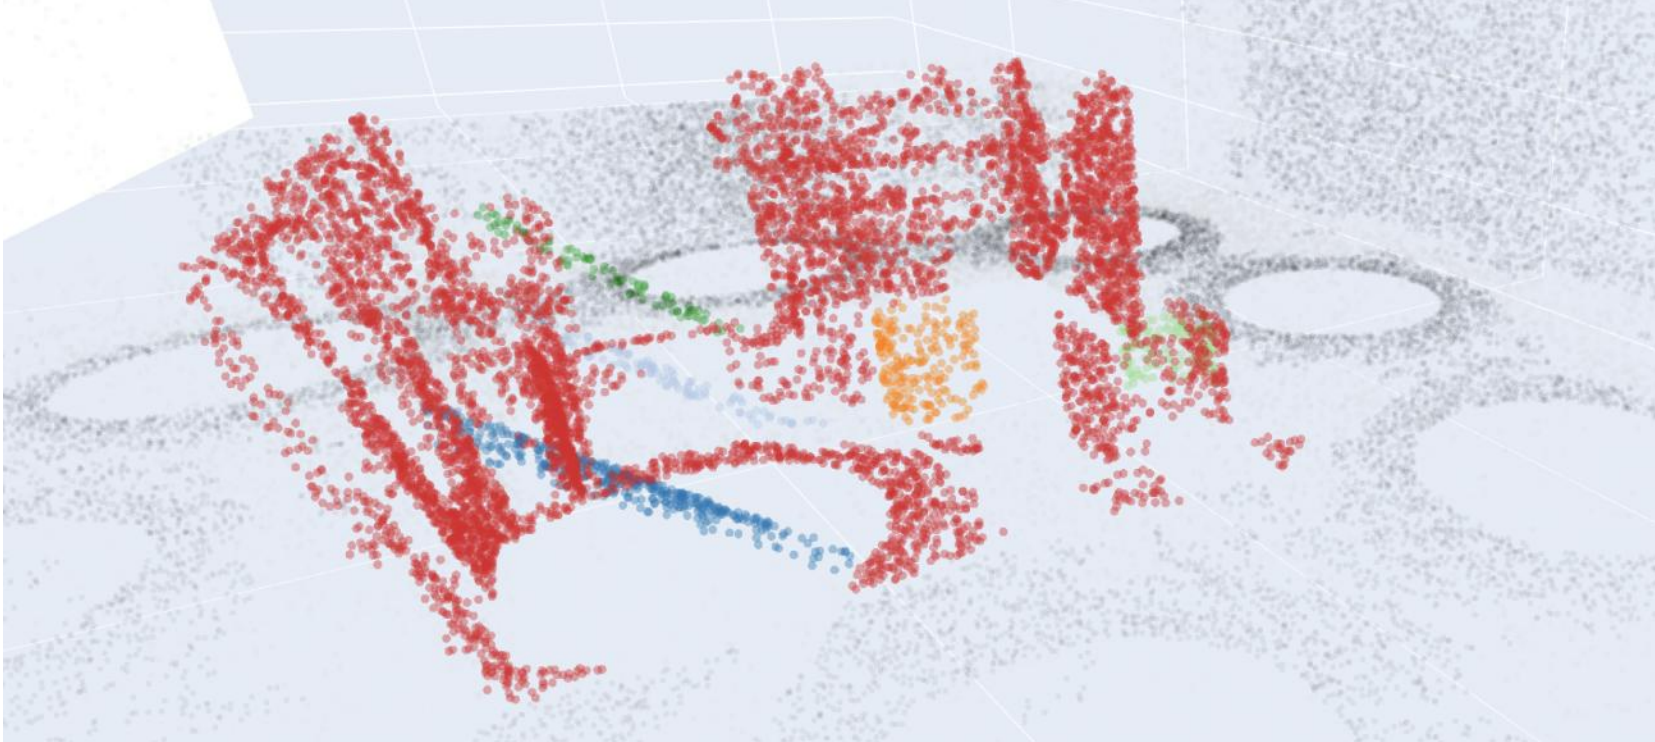
\includegraphics[width=\textwidth]{imgs/Resultat_MarieBenchmark.png}
                
                \vspace{0.3cm}
                \scriptsize \textbf{Résultat d'isolation d'anomalies} (modèle conforme en rouge, anomalies en couleurs distinctes).
            \end{center}
        \end{column}
    \end{columns}
\end{frame}

\begin{frame}{Segmentation d'instance sur LiDAR 3D/4D}
    \begin{columns}[c, onlytextwidth]
        \begin{column}{0.48\textwidth}
            \begin{itemize}
                \setlength{\itemsep}{12pt}
                \item \textbf{Perspectives industrielles} :
                \begin{itemize}
                    \item Collaborations et applications cibles avec Greehill, Valeo et Naval Group.
                \end{itemize}
                \item \textbf{Automatisation} :
                \begin{itemize}
                    \item Navigation pour véhicules autonomes et robotique mobile.
                \end{itemize}
                \item \textbf{Supervision \& Auscultation} :
                \begin{itemize}
                    \item Construction de jumeaux numériques urbains ou industriels.
                    \item Diagnostic de structures et détection précoce d'anomalies.
                \end{itemize}
            \end{itemize}
        \end{column}
        
        \begin{column}{0.48\textwidth}
            \begin{center}
                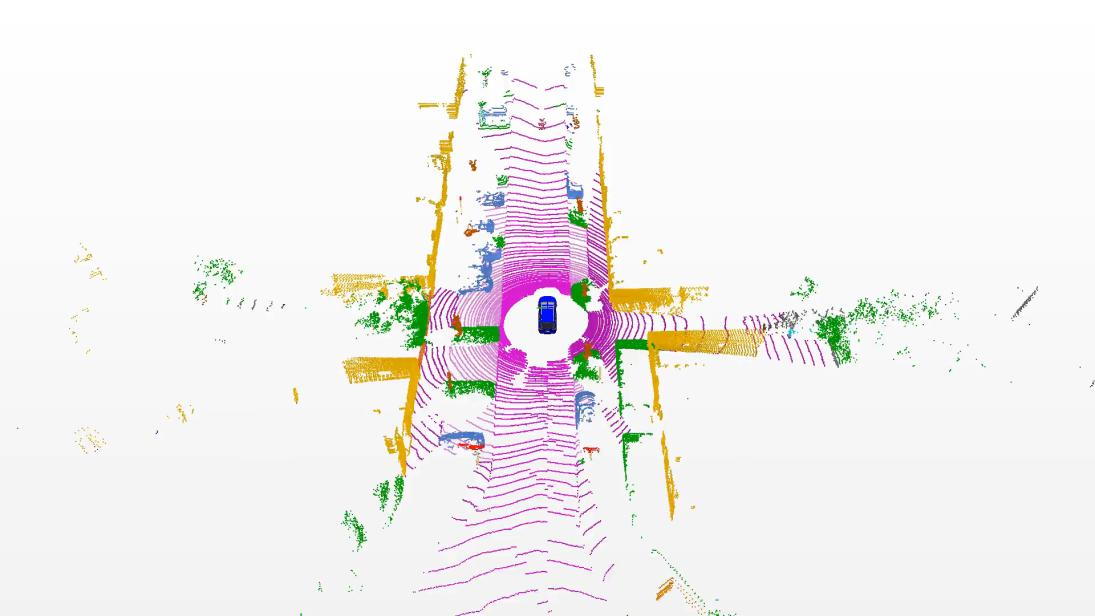
\includegraphics[width=0.95\textwidth]{imgs/liDAR_4D_industrials.jpg}
                
                \vspace{0.2cm}
                \scriptsize Scène LiDAR urbaine 3D dense.
            \end{center}
        \end{column}
    \end{columns}
\end{frame}

\begin{frame}{Segmentation panoptique LiDAR 3D : État de l'art}
    \begin{columns}[c, onlytextwidth]
        \begin{column}{0.50\textwidth}
            \begin{itemize}
                \setlength{\itemsep}{12pt}
                \item \textbf{Approche standard du domaine} :
                \begin{itemize}
                    \item Segmentation sémantique (Deep Learning) suivie d'un clustering spatial (DBSCAN / HDBSCAN).
                \end{itemize}
                \item \textbf{Limites majeures} :
                \begin{itemize}
                    \item Difficultés accrues du clustering dans les zones de forte densité ou sur les géométries complexes.
                \end{itemize}
                \item \textbf{Référence en 3D} :
                \begin{itemize}
                    \item \textbf{Alpine} \cite{Sautier2025} (\textsc{Sautier} \emph{et al.}, 2025) :
                    \item \emph{« Is clustering enough for LiDAR instance segmentation? »}
                \end{itemize}
            \end{itemize}
        \end{column}
        
        \begin{column}{0.46\textwidth}
            \begin{center}
                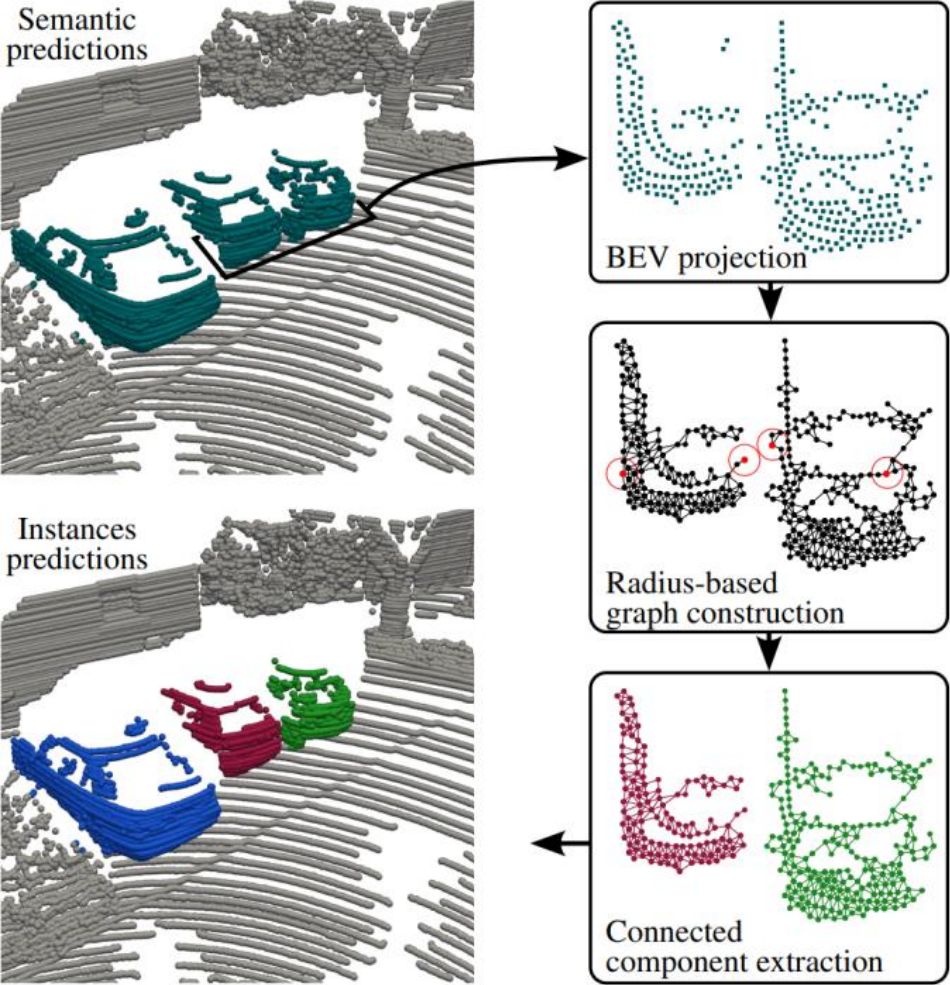
\includegraphics[height=0.75\textheight]{imgs/Alpine.png}
                
                \vspace{0.2cm}
                \scriptsize Visualisation d'instances détectées par Alpine.
            \end{center}
        \end{column}
    \end{columns}
\end{frame}

\begin{frame}{Segmentation panoptique LiDAR 4D : État de l'art}
    \begin{columns}[c, onlytextwidth]
        \begin{column}{0.50\textwidth}
            \begin{itemize}
                \setlength{\itemsep}{12pt}
                \item \textbf{Suivi temporel des objets (Tracking)} :
                \begin{itemize}
                    \item Association globale des instances sémantiques au cours du temps.
                \end{itemize}
                \item \textbf{Approche standard} :
                \begin{itemize}
                    \item Sémantique + Clustering + Association globale par Transport Optimal.
                \end{itemize}
                \item \textbf{Référence en 4D} :
                \begin{itemize}
                    \item \textbf{Geo-4D} \cite{Oh2025} (\textsc{Oh} \emph{et al.}, 2025) :
                    \item \emph{« Training-Free Global Geometric Association for 4D LiDAR Panoptic Segmentation »}.
                \end{itemize}
            \end{itemize}
        \end{column}
        
        \begin{column}{0.46\textwidth}
            \begin{center}
                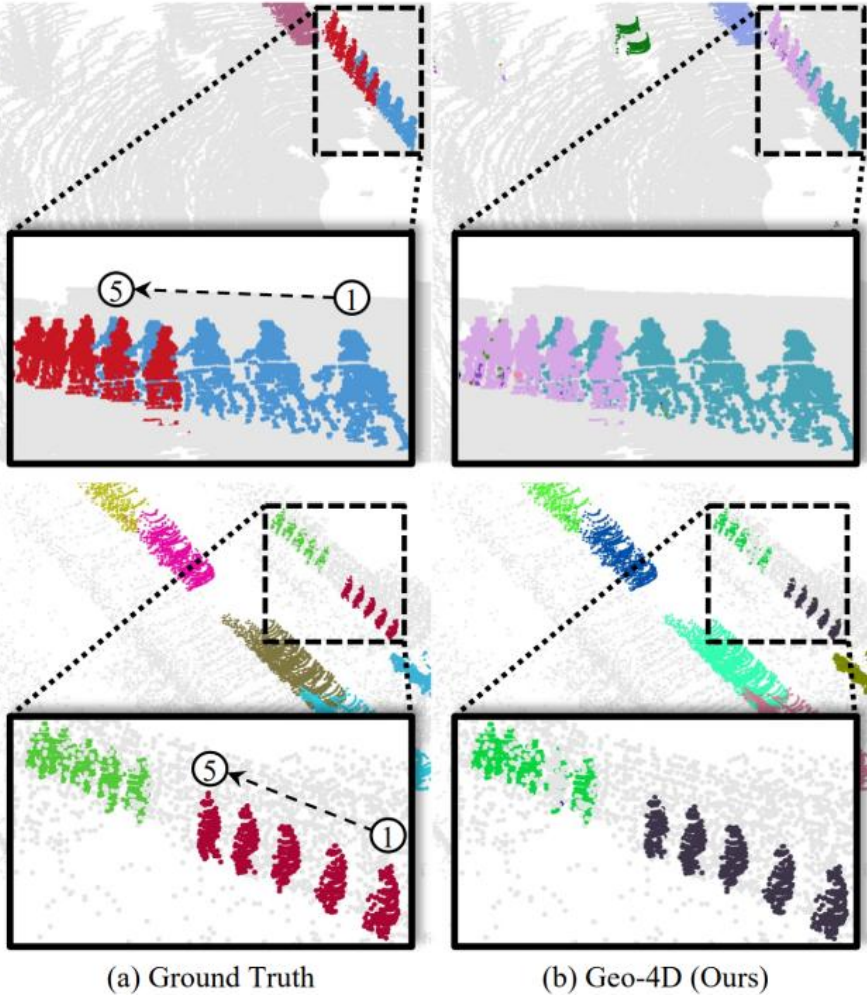
\includegraphics[height=0.75\textheight]{imgs/Resultat_Geo-4D.png}
                
                \vspace{0.2cm}
                \scriptsize Tracking temporel d'instances de véhicules dans Geo-4D.
            \end{center}
        \end{column}
    \end{columns}
\end{frame}

\begin{frame}{Segmentation d'instance 4D : Intégration d'a priori géométriques}
    \begin{columns}[c, onlytextwidth]
        \begin{column}{0.48\textwidth}
            \begin{itemize}
                \setlength{\itemsep}{14pt}
                \item \textbf{A priori géométriques faibles} :
                \begin{itemize}
                    \item Prise en compte du volume attendu (a priori faible) des objets d'intérêt (véhicules, piétons).
                \end{itemize}
                \item \textbf{Sélection dans l'arbre hiérarchique} :
                \begin{itemize}
                    \item Notre algorithme identifie les nœuds qui optimisent conjointement la densité spatiale et la contrainte de volume.
                \end{itemize}
            \end{itemize}
        \end{column}
        
        \begin{column}{0.48\textwidth}
            \begin{center}
                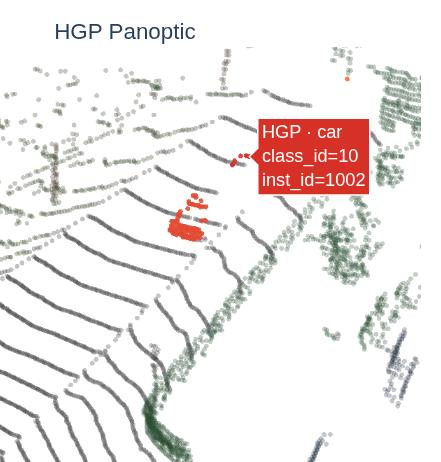
\includegraphics[width=0.48\textwidth]{imgs/kitti_3d_prior_1.jpg}
                \hfill
                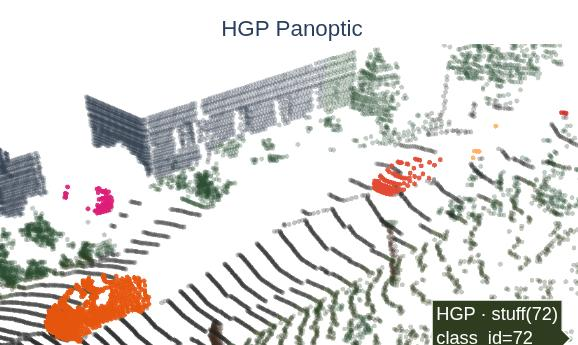
\includegraphics[width=0.48\textwidth]{imgs/kitti_3d_prior_2.jpg}
                
                \vspace{0.3cm}
                \scriptsize Exemples d'a priori géométriques appliqués aux volumes d'instances.
            \end{center}
        \end{column}
    \end{columns}
\end{frame}

\begin{frame}{Suivi temporel d'instance (SemanticKITTI)}
    \begin{columns}[c, onlytextwidth]
        \begin{column}{0.48\textwidth}
            \begin{itemize}
                \setlength{\itemsep}{14pt}
                \item \textbf{Association temporelle robuste} :
                \begin{itemize}
                    \item Suivi continu des instances à travers les frames successives.
                \end{itemize}
                \item \textbf{Reconstruction de trajectoires} :
                \begin{itemize}
                    \item Minimisation de l'erreur géométrique globale d'une frame à la suivante.
                \end{itemize}
            \end{itemize}
        \end{column}
        
        \begin{column}{0.48\textwidth}
            \begin{center}
                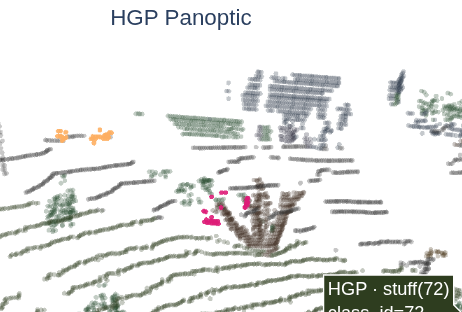
\includegraphics[width=0.95\textwidth]{imgs/kitti_3d_prior_3.png}
                
                \vspace{0.2cm}
                \scriptsize Trajectoires de véhicules estimées au cours du temps.
            \end{center}
        \end{column}
    \end{columns}
\end{frame}

\begin{frame}{Résultats de segmentation d'instance 4D}
    \begin{columns}[c, onlytextwidth]
        \begin{column}{0.35\textwidth}
            \begin{itemize}
                \setlength{\itemsep}{12pt}
                \item \textbf{Notre algorithme} :
                \begin{itemize}
                    \item Clustering hiérarchique d'ordre supérieur combiné au Transport Optimal non équilibré (\emph{unbalanced OT}).
                \end{itemize}
                \item \textbf{Sans entraînement} :
                \begin{itemize}
                    \item Résultats robustes s'affranchissant totalement de l'apprentissage profond pour la partie tracking et clustering.
                \end{itemize}
            \end{itemize}
        \end{column}
        
        \begin{column}{0.62\textwidth}
            \begin{center}
                \begin{tabular}{cc}
                    \textbf{Vérité terrain (GT)} & \textbf{Notre algorithme} \\
                    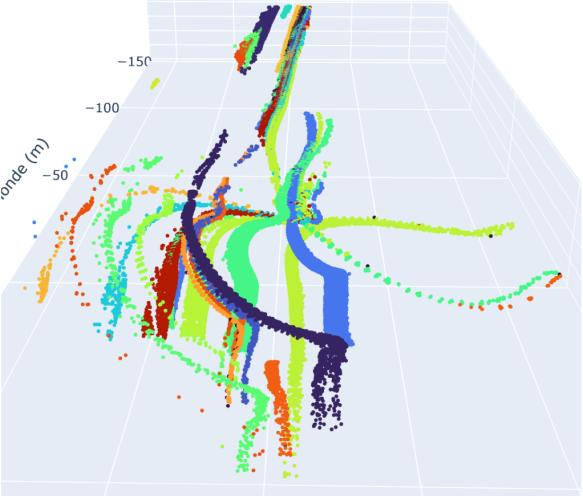
\includegraphics[width=0.46\textwidth]{imgs/kitti_ground_truth.jpg} &
                    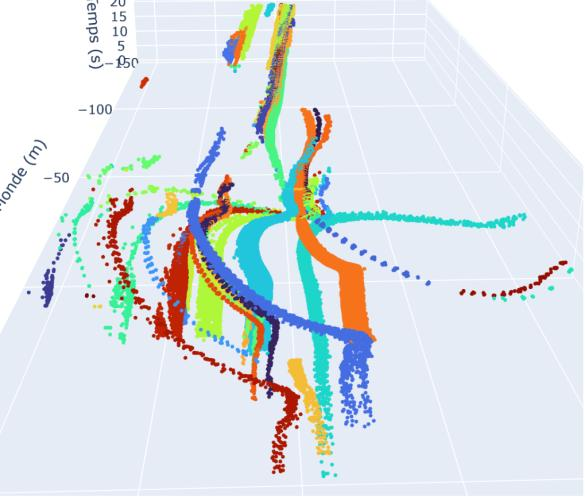
\includegraphics[width=0.46\textwidth]{imgs/kitti_our_algorithm.jpg}
                \end{tabular}
                
                \vspace{0.2cm}
                \scriptsize Comparaison visuelle des trajectoires reconstruites sur SemanticKITTI.
            \end{center}
        \end{column}
    \end{columns}
\end{frame}

\begin{frame}[allowframebreaks]{Références}
    \bibliographystyle{plain}
    \bibliography{referencesThesis}
\end{frame}

\end{document}
